% lfw.tex
%
% Author       : James Mnatzaganian, Qutaiba Saleh
% Date Created : 05/04/15
%
% Description  : LFW Paper
%
% Copyright (c) 2014 NanoComputing Research Lab

% Define the document type
\documentclass[10pt,journal]{IEEEtran}

% Packages
\usepackage{cite}                  % Citations
\usepackage[hidelinks]{hyperref}   % Links
\usepackage{graphicx}              % Figures
\usepackage{amsmath}               % Math
\usepackage{subcaption}            % Subcaptions
\usepackage[keeplastbox]{flushend} % Even column height at end

% Package configuration
\graphicspath{{figures/}}

% Macros
\newcommand{\fig}[1]{Fig.~\ref{#1}}
\newcommand{\subfig}[1]{~(\ref{#1})}
\newcommand{\eq}[1]{(\ref{#1})}
\newcommand{\tbl}[1]{Table~\ref{#1}}

% Add DRAFT to the document
% \usepackage{watermark}
% \watermark{\hspace{-0.3in} \textbf{DRAFT} \hspace{2.0in} \textbf{\today}}

\begin{document}
	
	\title{An Efficient Hardware Implementation of Competitive Learning Classifier for Gender Classification}
	
	\author{
		James~Mnatzaganian,~\IEEEmembership{Student Member,~IEEE,}
        and~Qutaiba~Saleh,~\IEEEmembership{Student Member,~IEEE}%
	
		\IEEEcompsocitemizethanks{
			\IEEEcompsocthanksitem J. Mnatzaganian, and Q. Saleh are with the NanoComputing Research Laboratory, Rochester Institute of Technology, Rochester, NY, 14623.
		}%
		
		\thanks{Manuscript received May 21, 2015.}
	}
	
	% \markboth{Journal of IEEE Transactions,~Vol.~?, No.~?, ?~2015}%
	
	\IEEEtitleabstractindextext{%
		\begin{abstract}
			A Competitive Learning Classifier (CLC) is introduced as a suitable algorithm for performing real-time gender classification in embedded applications. CLC is a type of clustering algorithm, derived from competitive learning. The design was able to obtain an accuracy of up to 70~\%. The hardware could perform training and testing operations at a rate of at least 25~MHz. The design footprint was 0.0176 mm\textsuperscript{2} and consumed only 1.1 mW of power per epoch per 800 training and 1000 testing patterns. Due to the low power consumption, small footprint, and fast operation this design is suitable for real-time embedded applications.
		\end{abstract}
	
	\begin{IEEEkeywords}
		Competitive Learning Classifier (CLC), gender classification, ASIC, low power.
	\end{IEEEkeywords}}

	\maketitle
	\IEEEdisplaynontitleabstractindextext
	
	\IEEEPARstart{G}{ender}
		classification is an important topic in social interactions. It can determine the greeting from one individual to another as well as the entire context of the conversation. Additionally, determining an individual's gender could be used to market products specifically for that gender. For example, a clothing store could have an automated advertising board to display products that would best suit the individual entering their store. If a gender detection system was being used in that manner, the system would need to be able to determine the gender classification in real-time, additionally it should consume as little power as possible.
		
		This problem has been explored by many software approaches (e.g.~\cite{sw_comparison,sw_svm,sw_cnn}), but only a couple hardware implementations exist~\cite{ann_fpga,svm_fpga}. For a real-time embedded system, the design should ideally be a low-power ASIC. None of the past designs created an ASIC and additionally none of those designs mentioned power consumption. This work developed a custom algorithm explicitly designed to be as efficient as possible while still achieving acceptable accuracies.
		
		% Belongs to Design Approach -> Algorithm section
		\begin{figure}
			\centering
			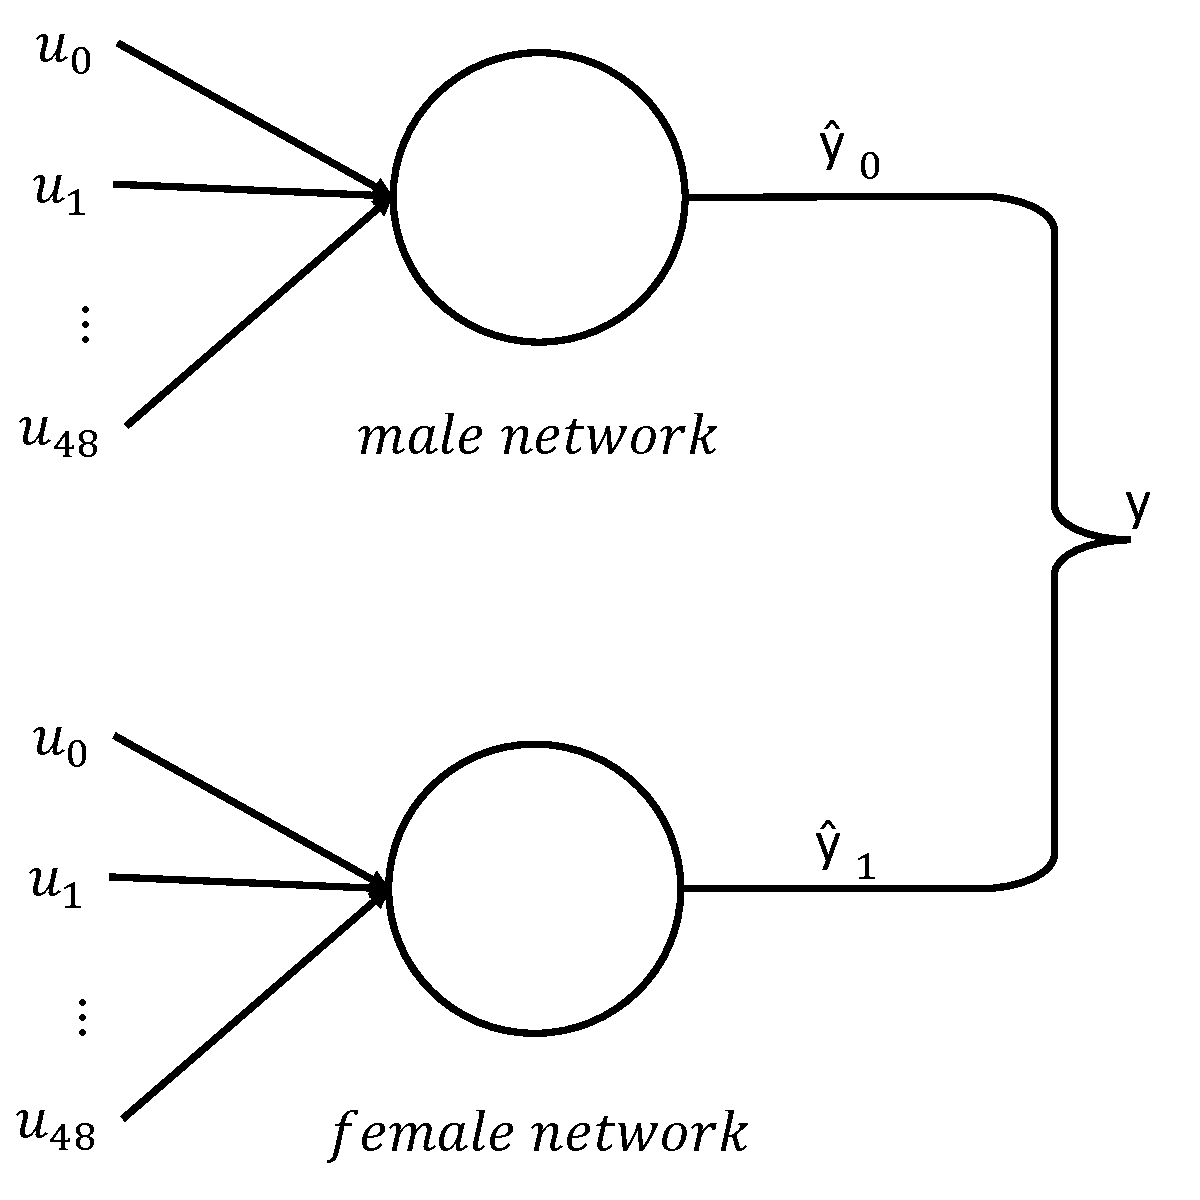
\includegraphics[width=0.8\linewidth]{network}
			\caption{A CLC consisting of two networks (male and female), 49 inputs per network, and a single output for each network.}
			\label{fig:network}
		\end{figure}
	
	\subsection{Dataset}
		The Labeled Faces in the Wild (LFW)~\cite{lfw} dataset was modified for use with gender classification. This dataset is comprised of one or more faces per person, with no labels to denote gender. To obtain the genders, the genderize.io~\cite{genderize} API was utilized. This API can be used to obtain the gender, with a confidence interval, for a given first name. Only results with over 90\% accuracy were utilized.
		
		The faces in the dataset are not all frontalized nor are they cropped to remove background noise. To remove noise, the frontalized images from Hassner et al.~\cite{frontalize} were used as the dataset. This dataset frontalized and cropped all images from the LFW dataset, creating a cleaner dataset. The images were then resized to various sizes using bilinear interpolation. The raw pixels were then used as the features.
		
		To ensure that the dataset would not be biased towards a particular individual, a single instance of each person was randomly chosen. The remaining images were then randomized and split by gender, to ensure an equal distribution of males and females. 400 of each gender were used for training and 200 of each gender were used for testing. All code for generating the dataset as well as the software and hardware models are available at~\cite{gitrepo}.
	
	\subsection{Design Approach}
		The primary design constraints were area and power. With this in mind, the system still had to perform its primary goal of gender classification. It was desired to obtain the highest possible accuracy; however, if a minor loss in accuracy resulted in major hardware improvements, favor was given to the hardware.
		
		\subsubsection{Algorithm}
			% Belongs to Software -> Parameter Optimization section
			\begin{figure*}[t!]
				\captionsetup[subfigure]{position=b}
				\centering
				\hfill
				\subcaptionbox
				{
					Training results
					\label{fig:sw_img:training}
				}
				{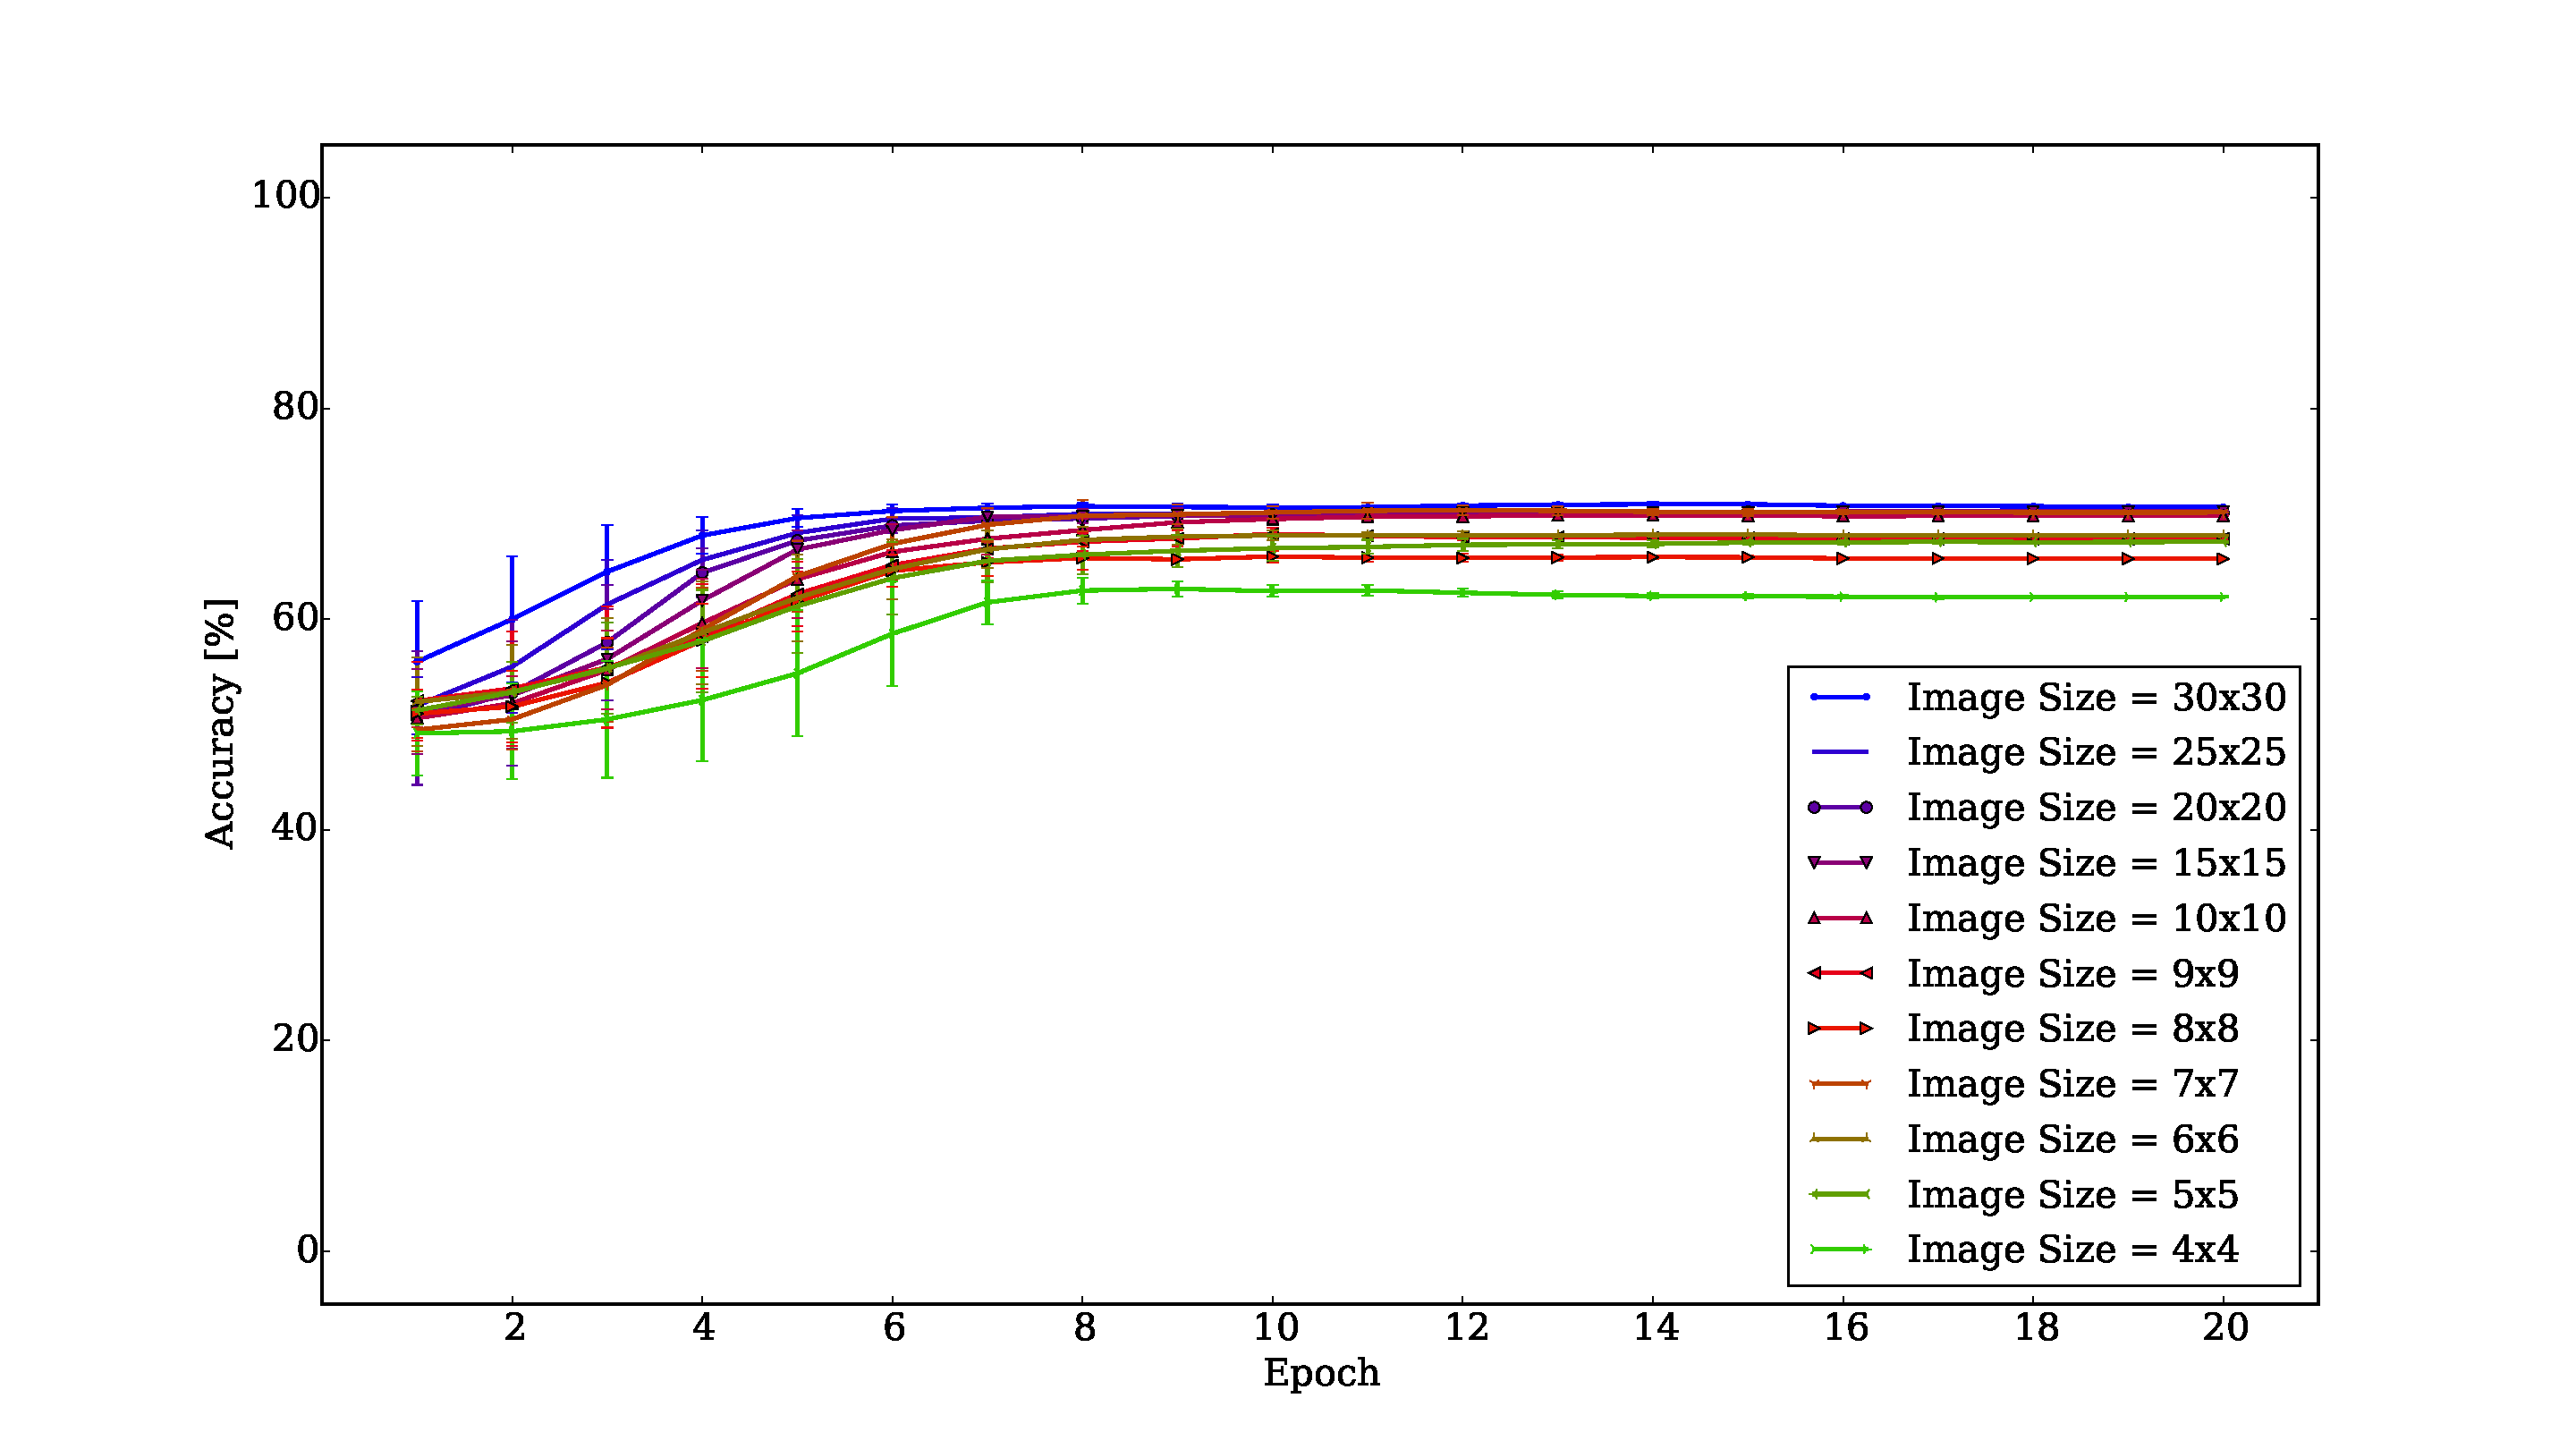
\includegraphics[width=0.49\linewidth]{sw_img_training}}
				\hfill
				\subcaptionbox
				{
					Testing results
					\label{fig:sw_img:testing}
				}
				{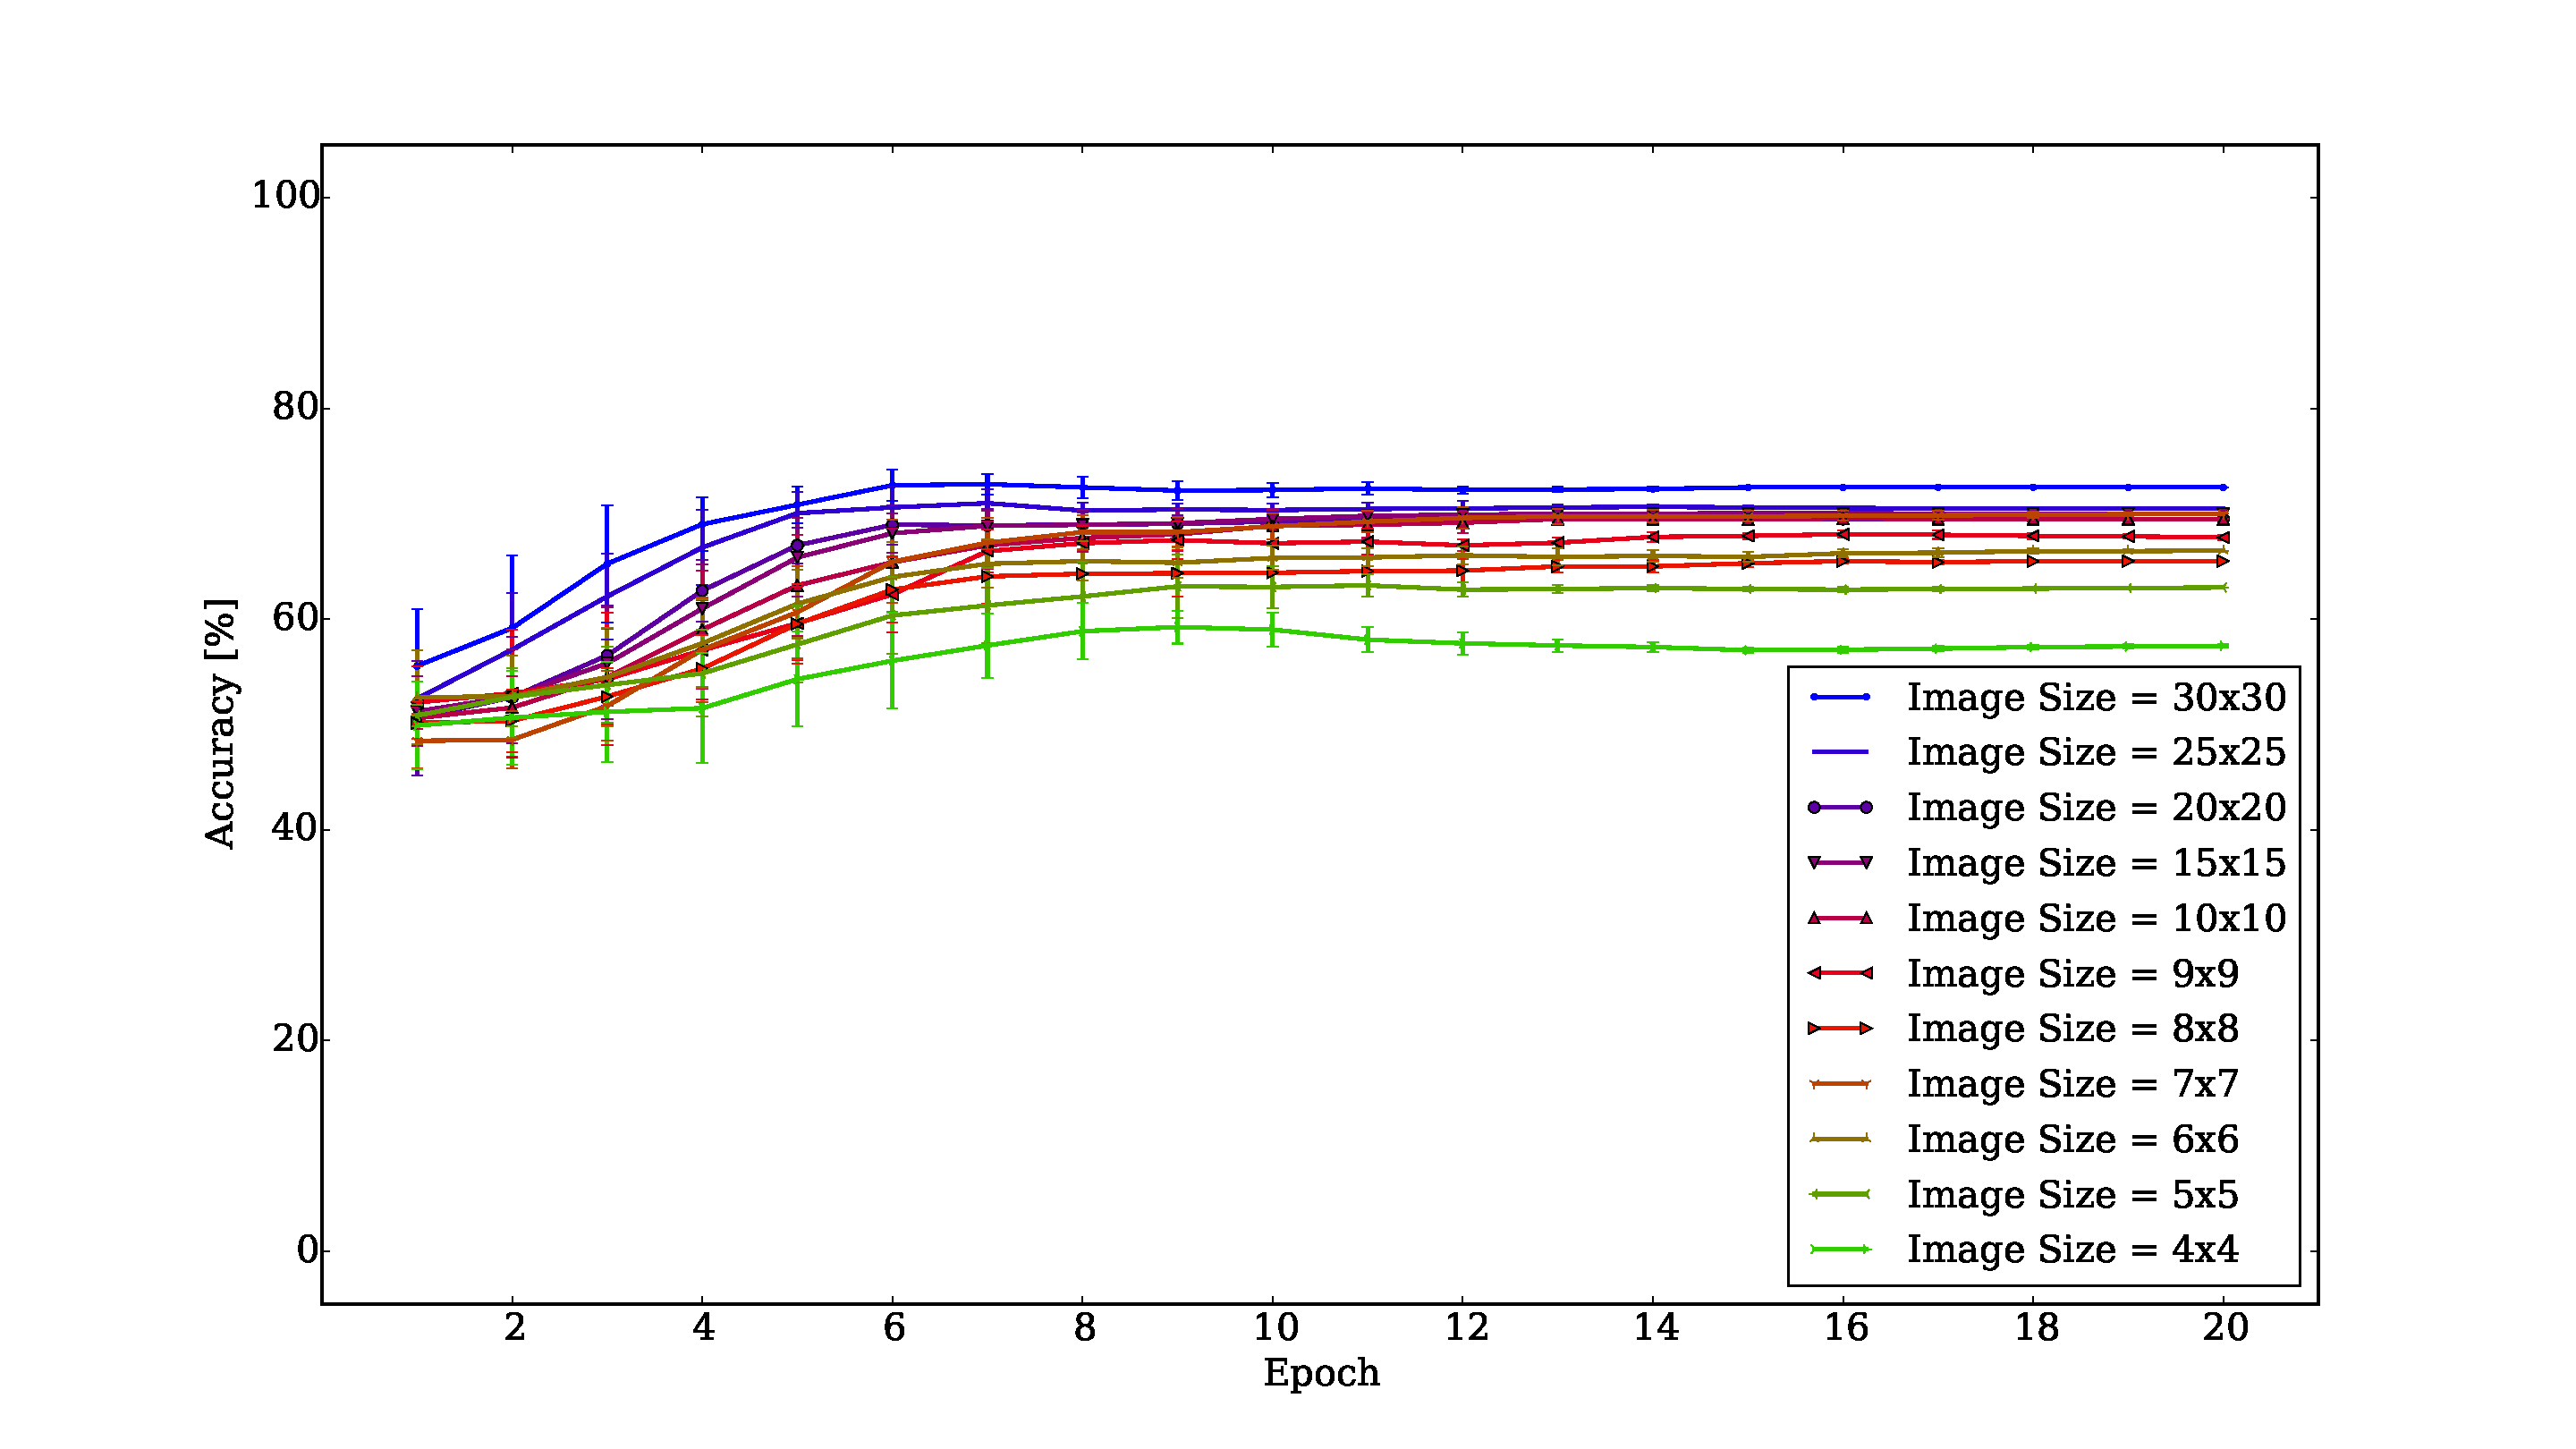
\includegraphics[width=0.49\linewidth]{sw_img_testing}}
				\hfill
				\caption{Training\subfig{fig:sw_img:training} and testing\subfig{fig:sw_img:testing} results for various image sizes. Each network has a single output. The learning rate was set to 0.001.}
				\label{fig:sw_img}
			\end{figure*}
			
			An algorithm similar to competitive learning was designed. This algorithm is coined Competitive Learning Classifier (CLC). The algorithm is comprised of \(N\) competitive learning networks, where \(N\) is the number of labels. Each network has \(I\) inputs and \(O\) outputs, where each output represents a cluster. The implementation of this algorithm used for this work is shown in \fig{fig:network}. It consists of two competitive learning networks (one for males and one for females), 49 inputs per network (one for each feature), and a single output for each network.
			
			\begin{equation}
				\label{sw_weight_update}
				\Delta w_{i,n} = \alpha\hat{y}_{o,n}^{(p)}(u_i^{(p)}-w_{i,n})
			\end{equation}
			
			\begin{equation}
				\label{sw_output}
				\hat{y}_{o,n}^{(p)} = \displaystyle\sum_{i=1}^{I}(w_{i,n} - u_i^{(p)})^2
			\end{equation}
			
			\begin{equation}
				\label{cost_function}
				J(\boldsymbol{w}_n) = \cfrac{1}{2}\displaystyle\sum_{p=1}^{P}\displaystyle\sum_{o=1}^{O}\hat{y}_{o,n}^{(p)}|\boldsymbol{w}_n-\boldsymbol{u}^{(p)}|^2
			\end{equation}
			
			In CLC, there is a randomly initialized weight for each input in each network. The weights are updated using the online update equation in \eq{sw_weight_update}, where \(w_{i,n}\) is the weight of input \(i\) for network \(n\), \(\alpha\) is the learning rate, \(\hat{y}_{o,n}^{(p)}\) is output \(o\) of network \(n\) for pattern \(p\), and \(u_i^{(p)}\) is input \(i\) for pattern \(p\). Each output is computed by finding the squared Euclidean distance between the weight and the input, as shown in \eq{sw_output}. The corresponding cost function is shown in \eq{cost_function}, where \(P\) is the total number of patterns.
			
			If \(O>1\) dead neurons may occur. To combat this, boosting is used, where frequently winning neurons are negatively boosted and infrequently winning neurons are positively boosted. Boosting is only updated during the learning phase, so after training the boost values are fixed.
			
			Training occurs by selecting the network representing the current label and updating its weights. The other networks are left untouched. During testing, both networks receive the same input and compute their respective outputs. The neuron having the lowest value is the winning neuron and the network that it belongs to becomes the output of the network.
			
		
		\subsubsection{Software}
			The software design consisted of two phases. The first phase involved finding a set of parameters that would obtain suitable accuracies. Additionally, those parameters should be tweaked, if possible, to simplify the hardware. The second phase involved redesigning the CLC model to be identical to the hardware design. This includes any simplifications as well as performing calculations using the same precision that would be used in the hardware.
			
			\paragraph{Parameter Optimization}
				\begin{figure*}[t!]
					\captionsetup[subfigure]{position=b}
					\centering
					\hfill
					\subcaptionbox
					{
						Training results
						\label{fig:sw_outputs:training}
					}
					{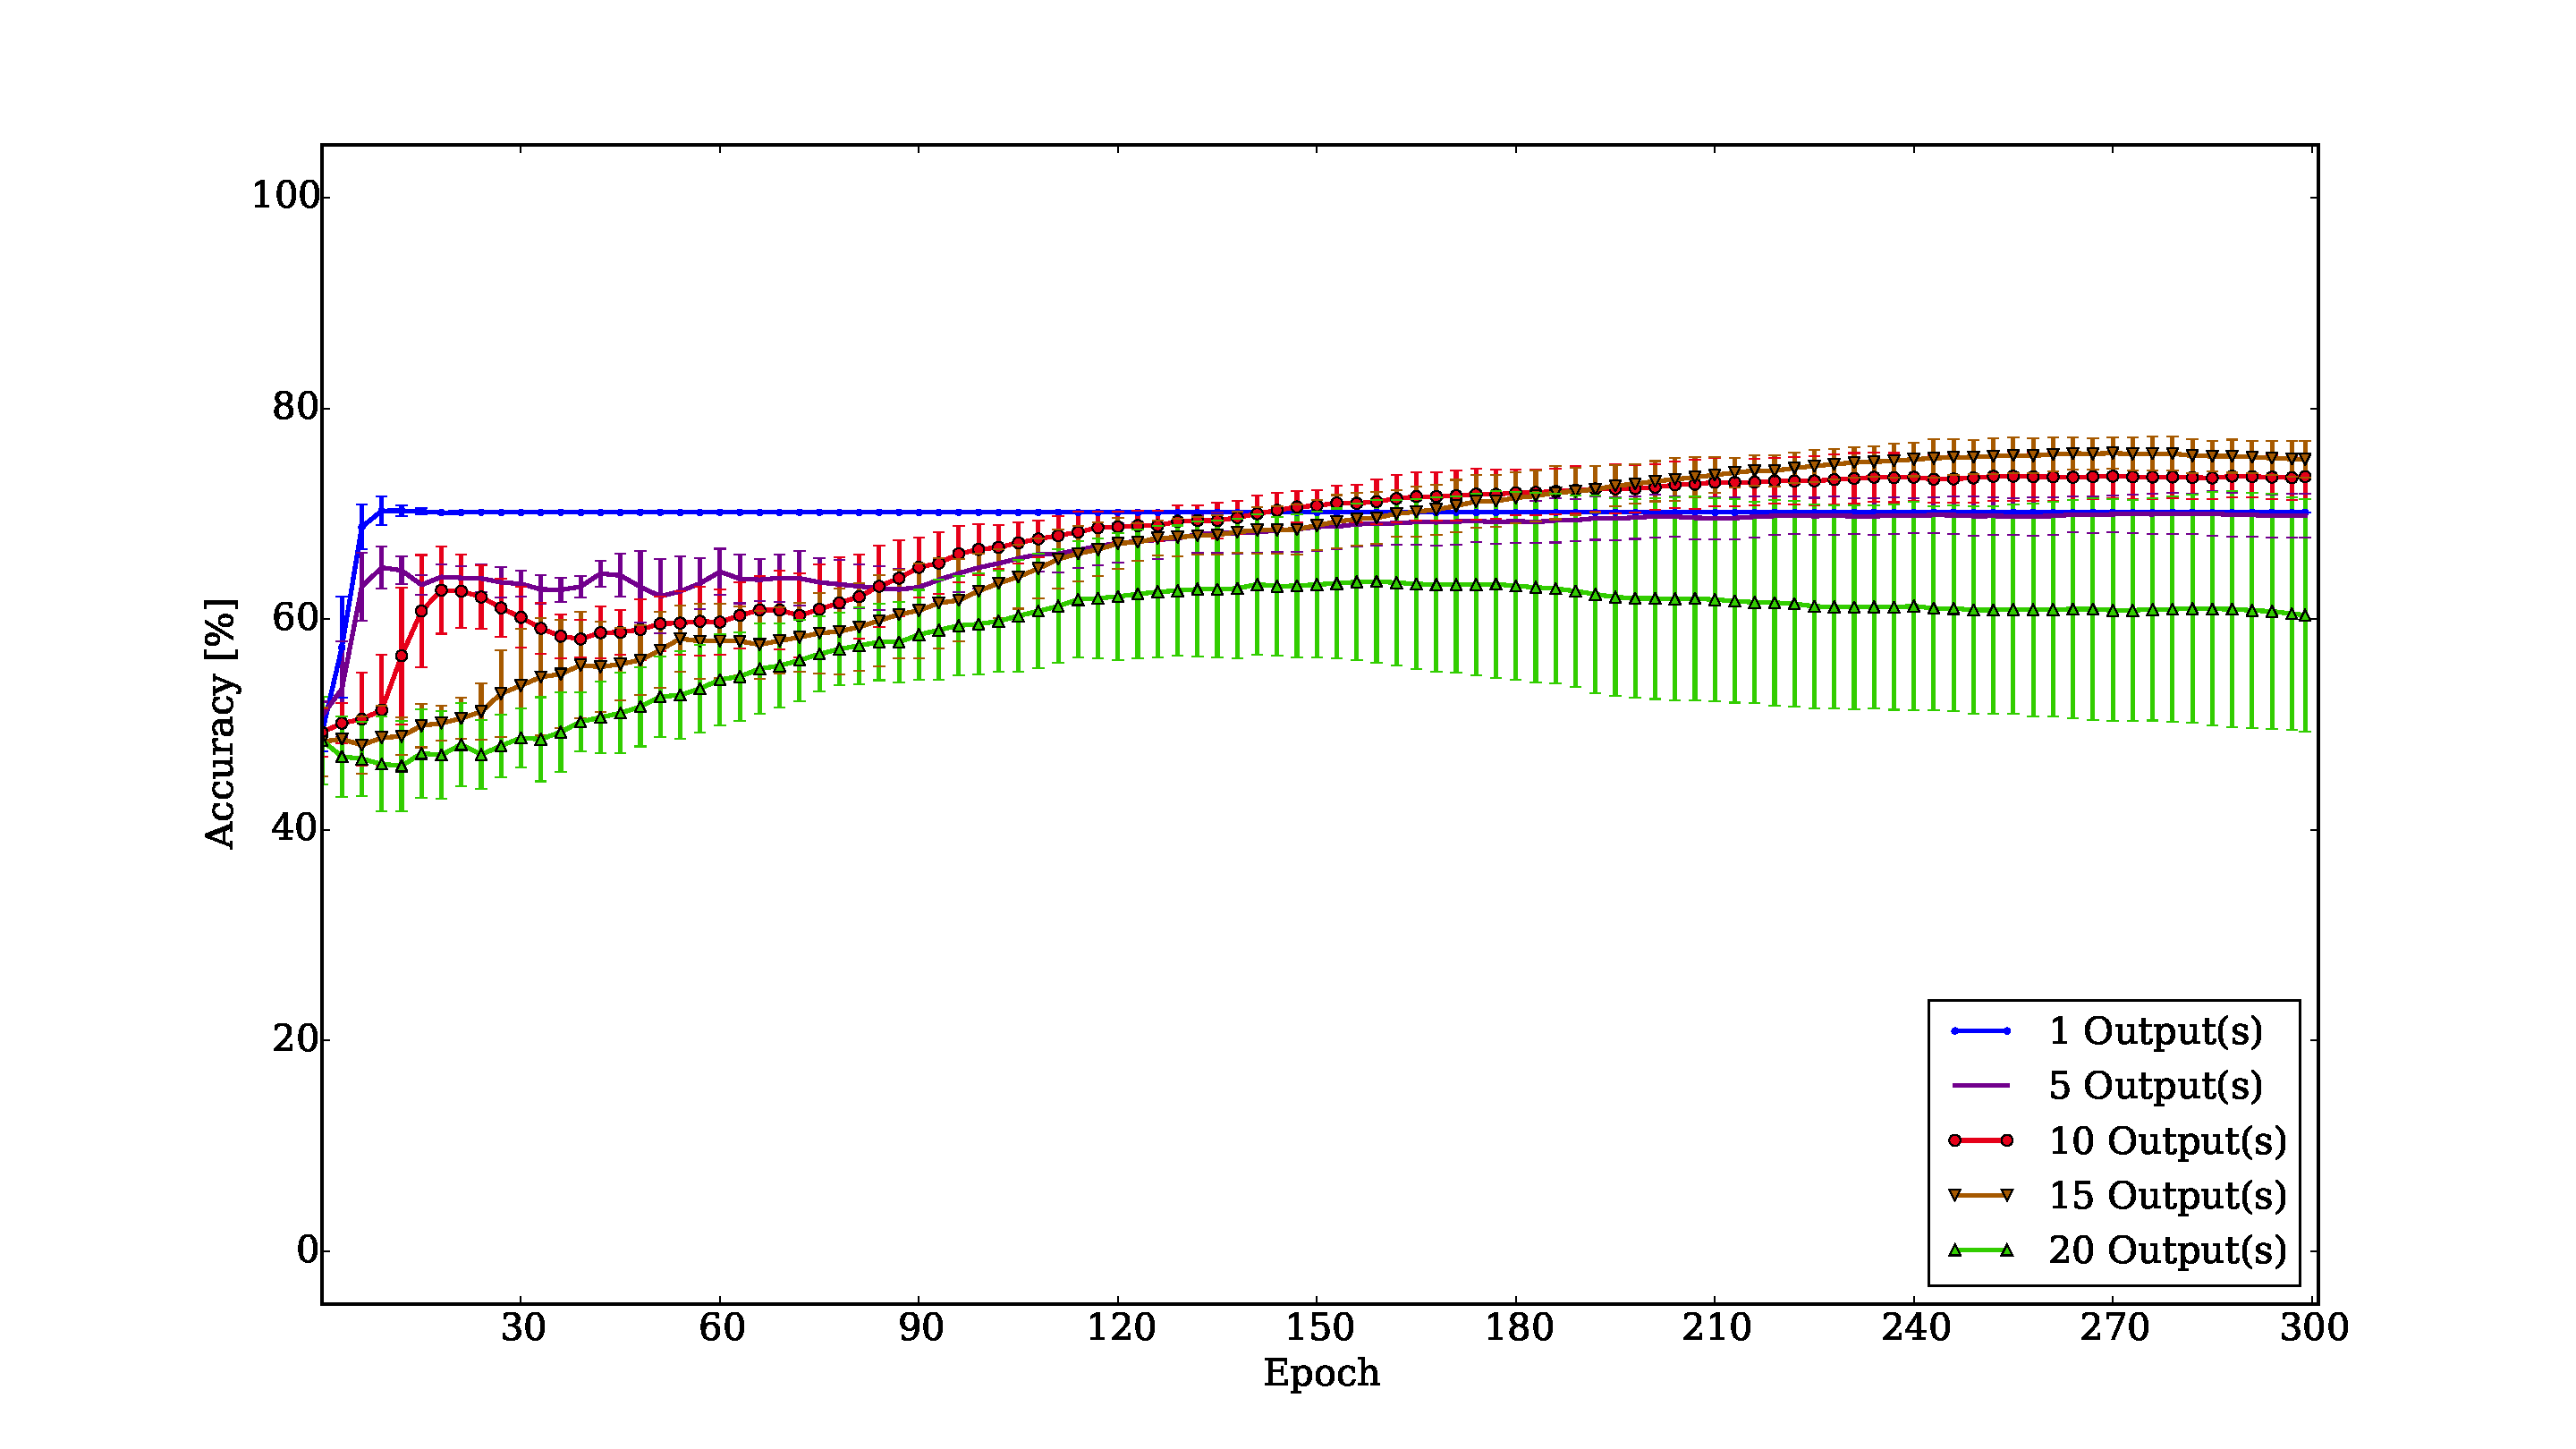
\includegraphics[width=0.49\linewidth]{sw_outputs_training}}
					\hfill
					\subcaptionbox
					{
						Testing results
						\label{fig:sw_outputs:testing}
					}
					{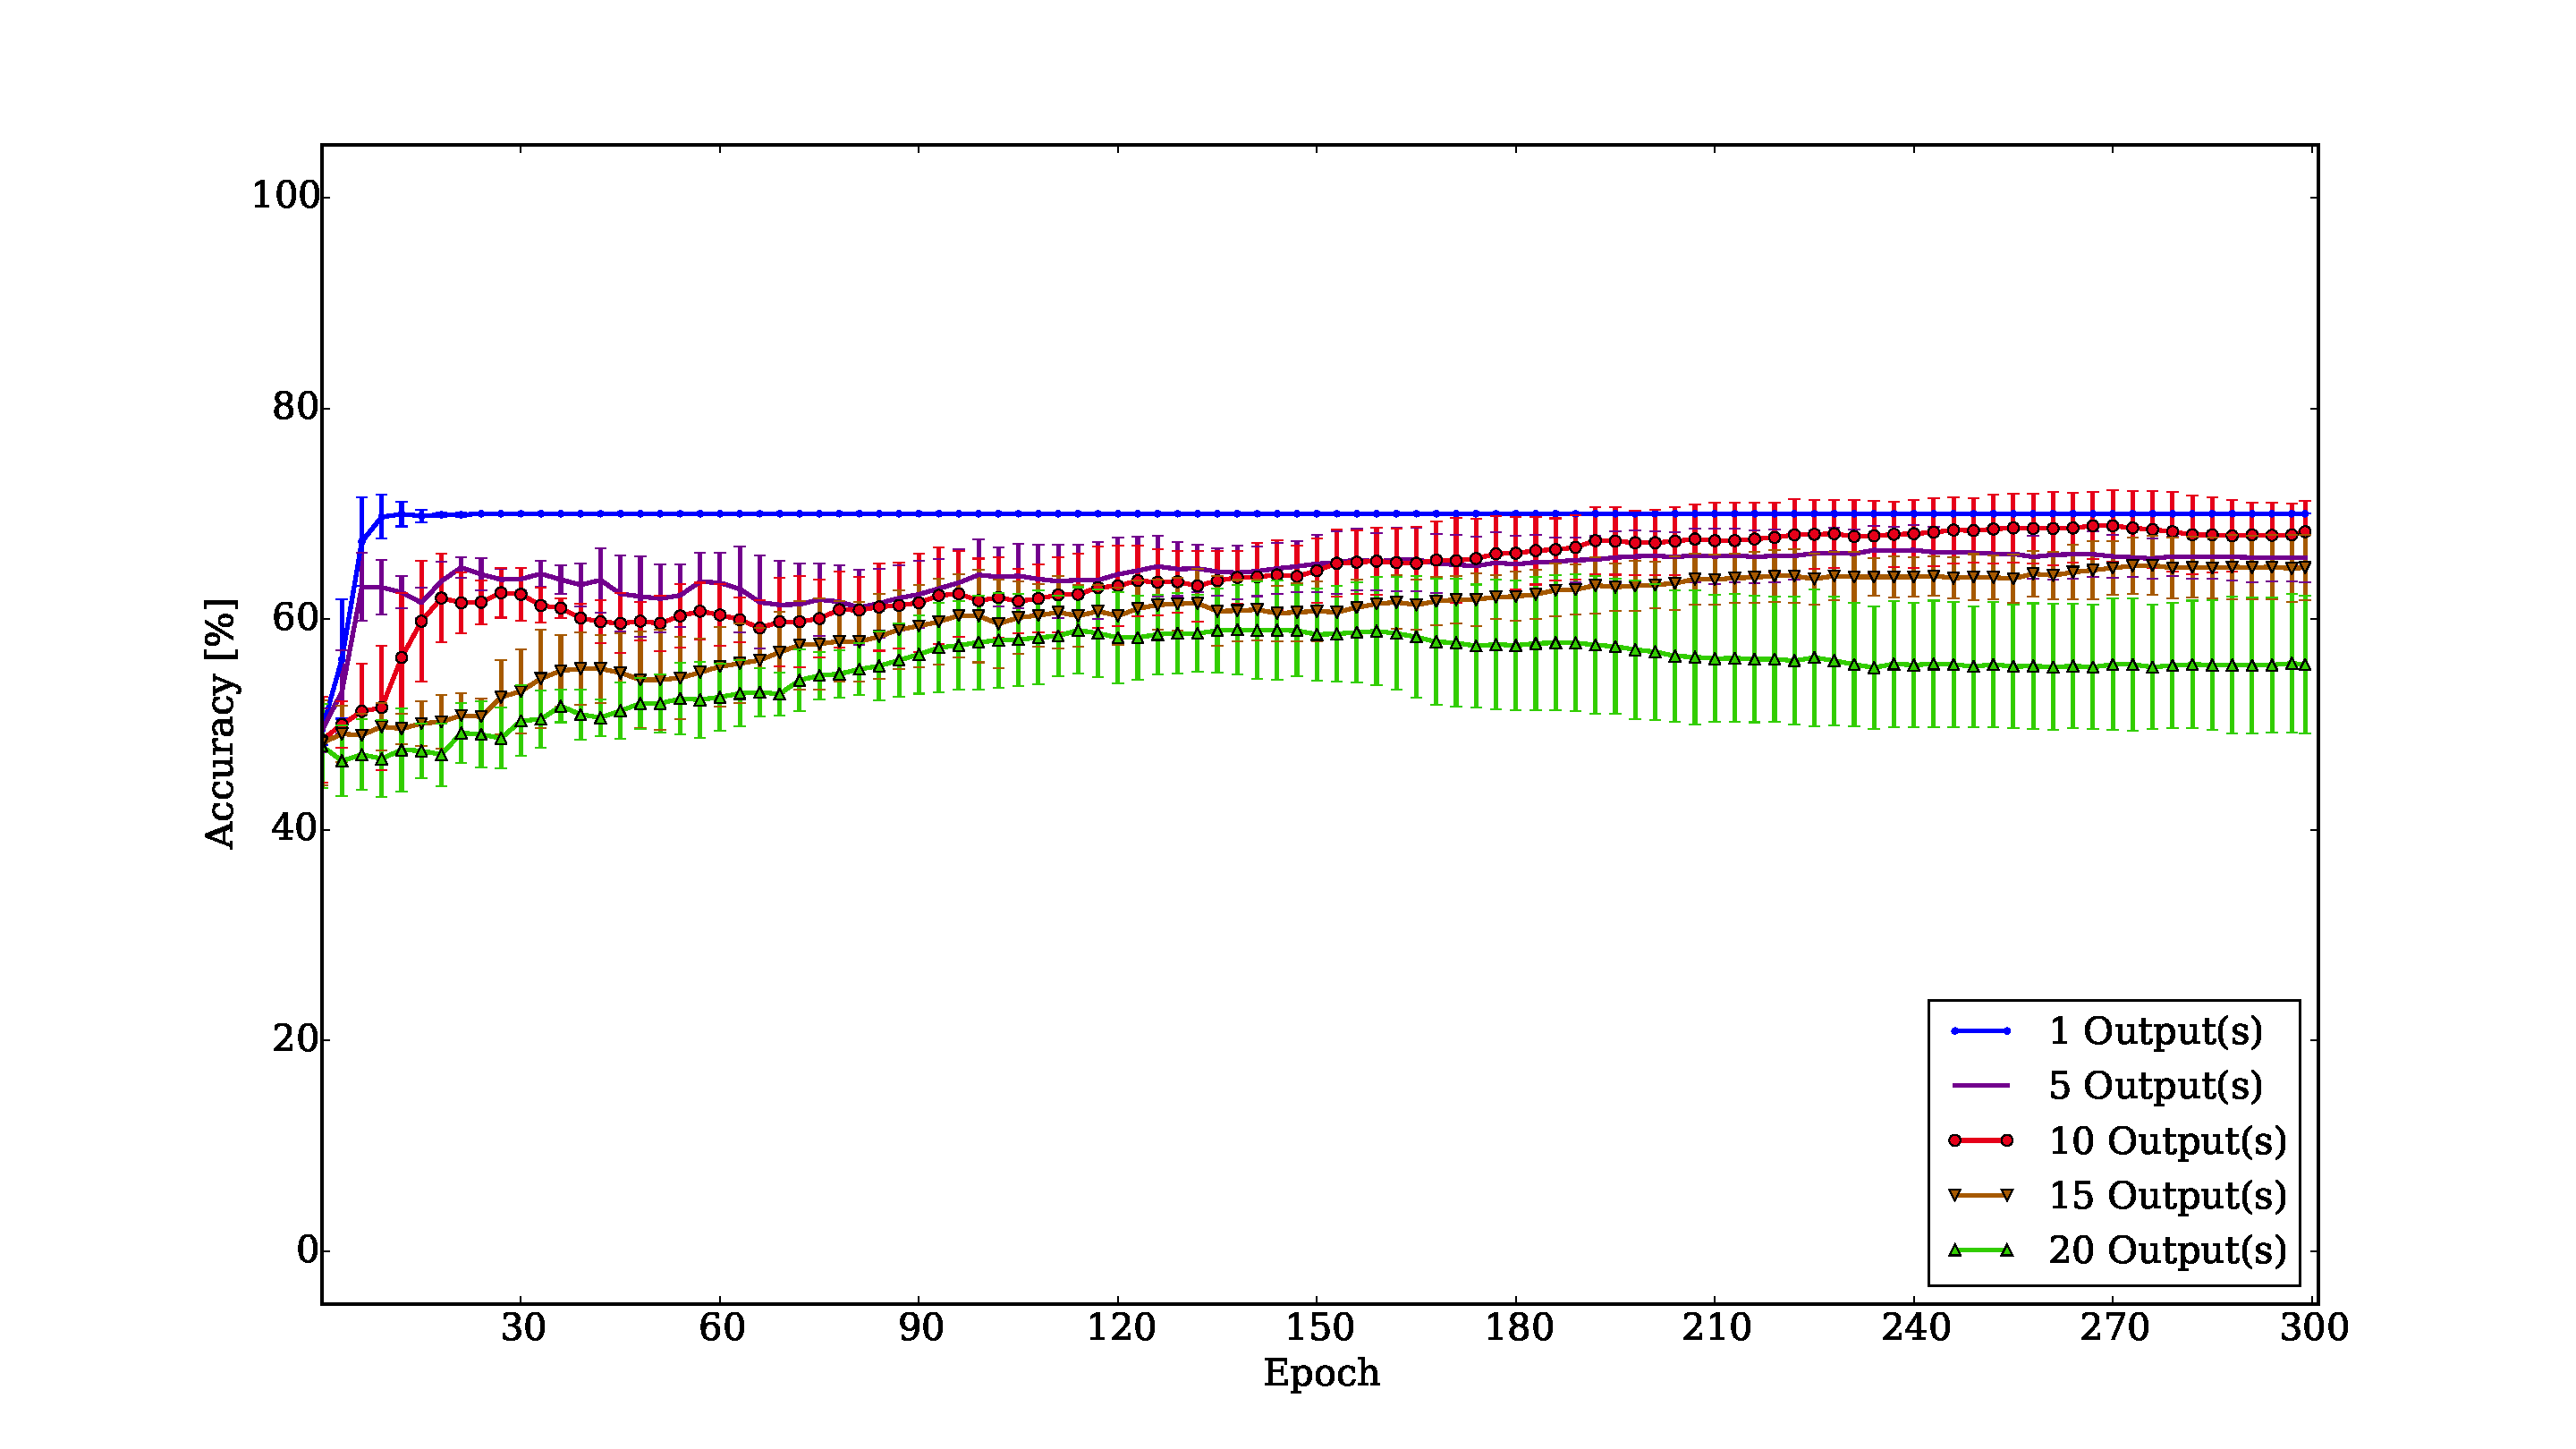
\includegraphics[width=0.49\linewidth]{sw_outputs_testing}}
					\hfill
					\caption{Training\subfig{fig:sw_outputs:training} and testing\subfig{fig:sw_outputs:testing} results for a various number of network outputs. The image size was 7x7. The learning rate was set to 0.001.}
					\label{fig:sw_outputs}
				\end{figure*}
				
				\begin{figure*}[t!]
					\captionsetup[subfigure]{position=b}
					\centering
					\hfill
					\subcaptionbox
					{
						Training results
						\label{fig:sw_learning_rate:training}
					}
					{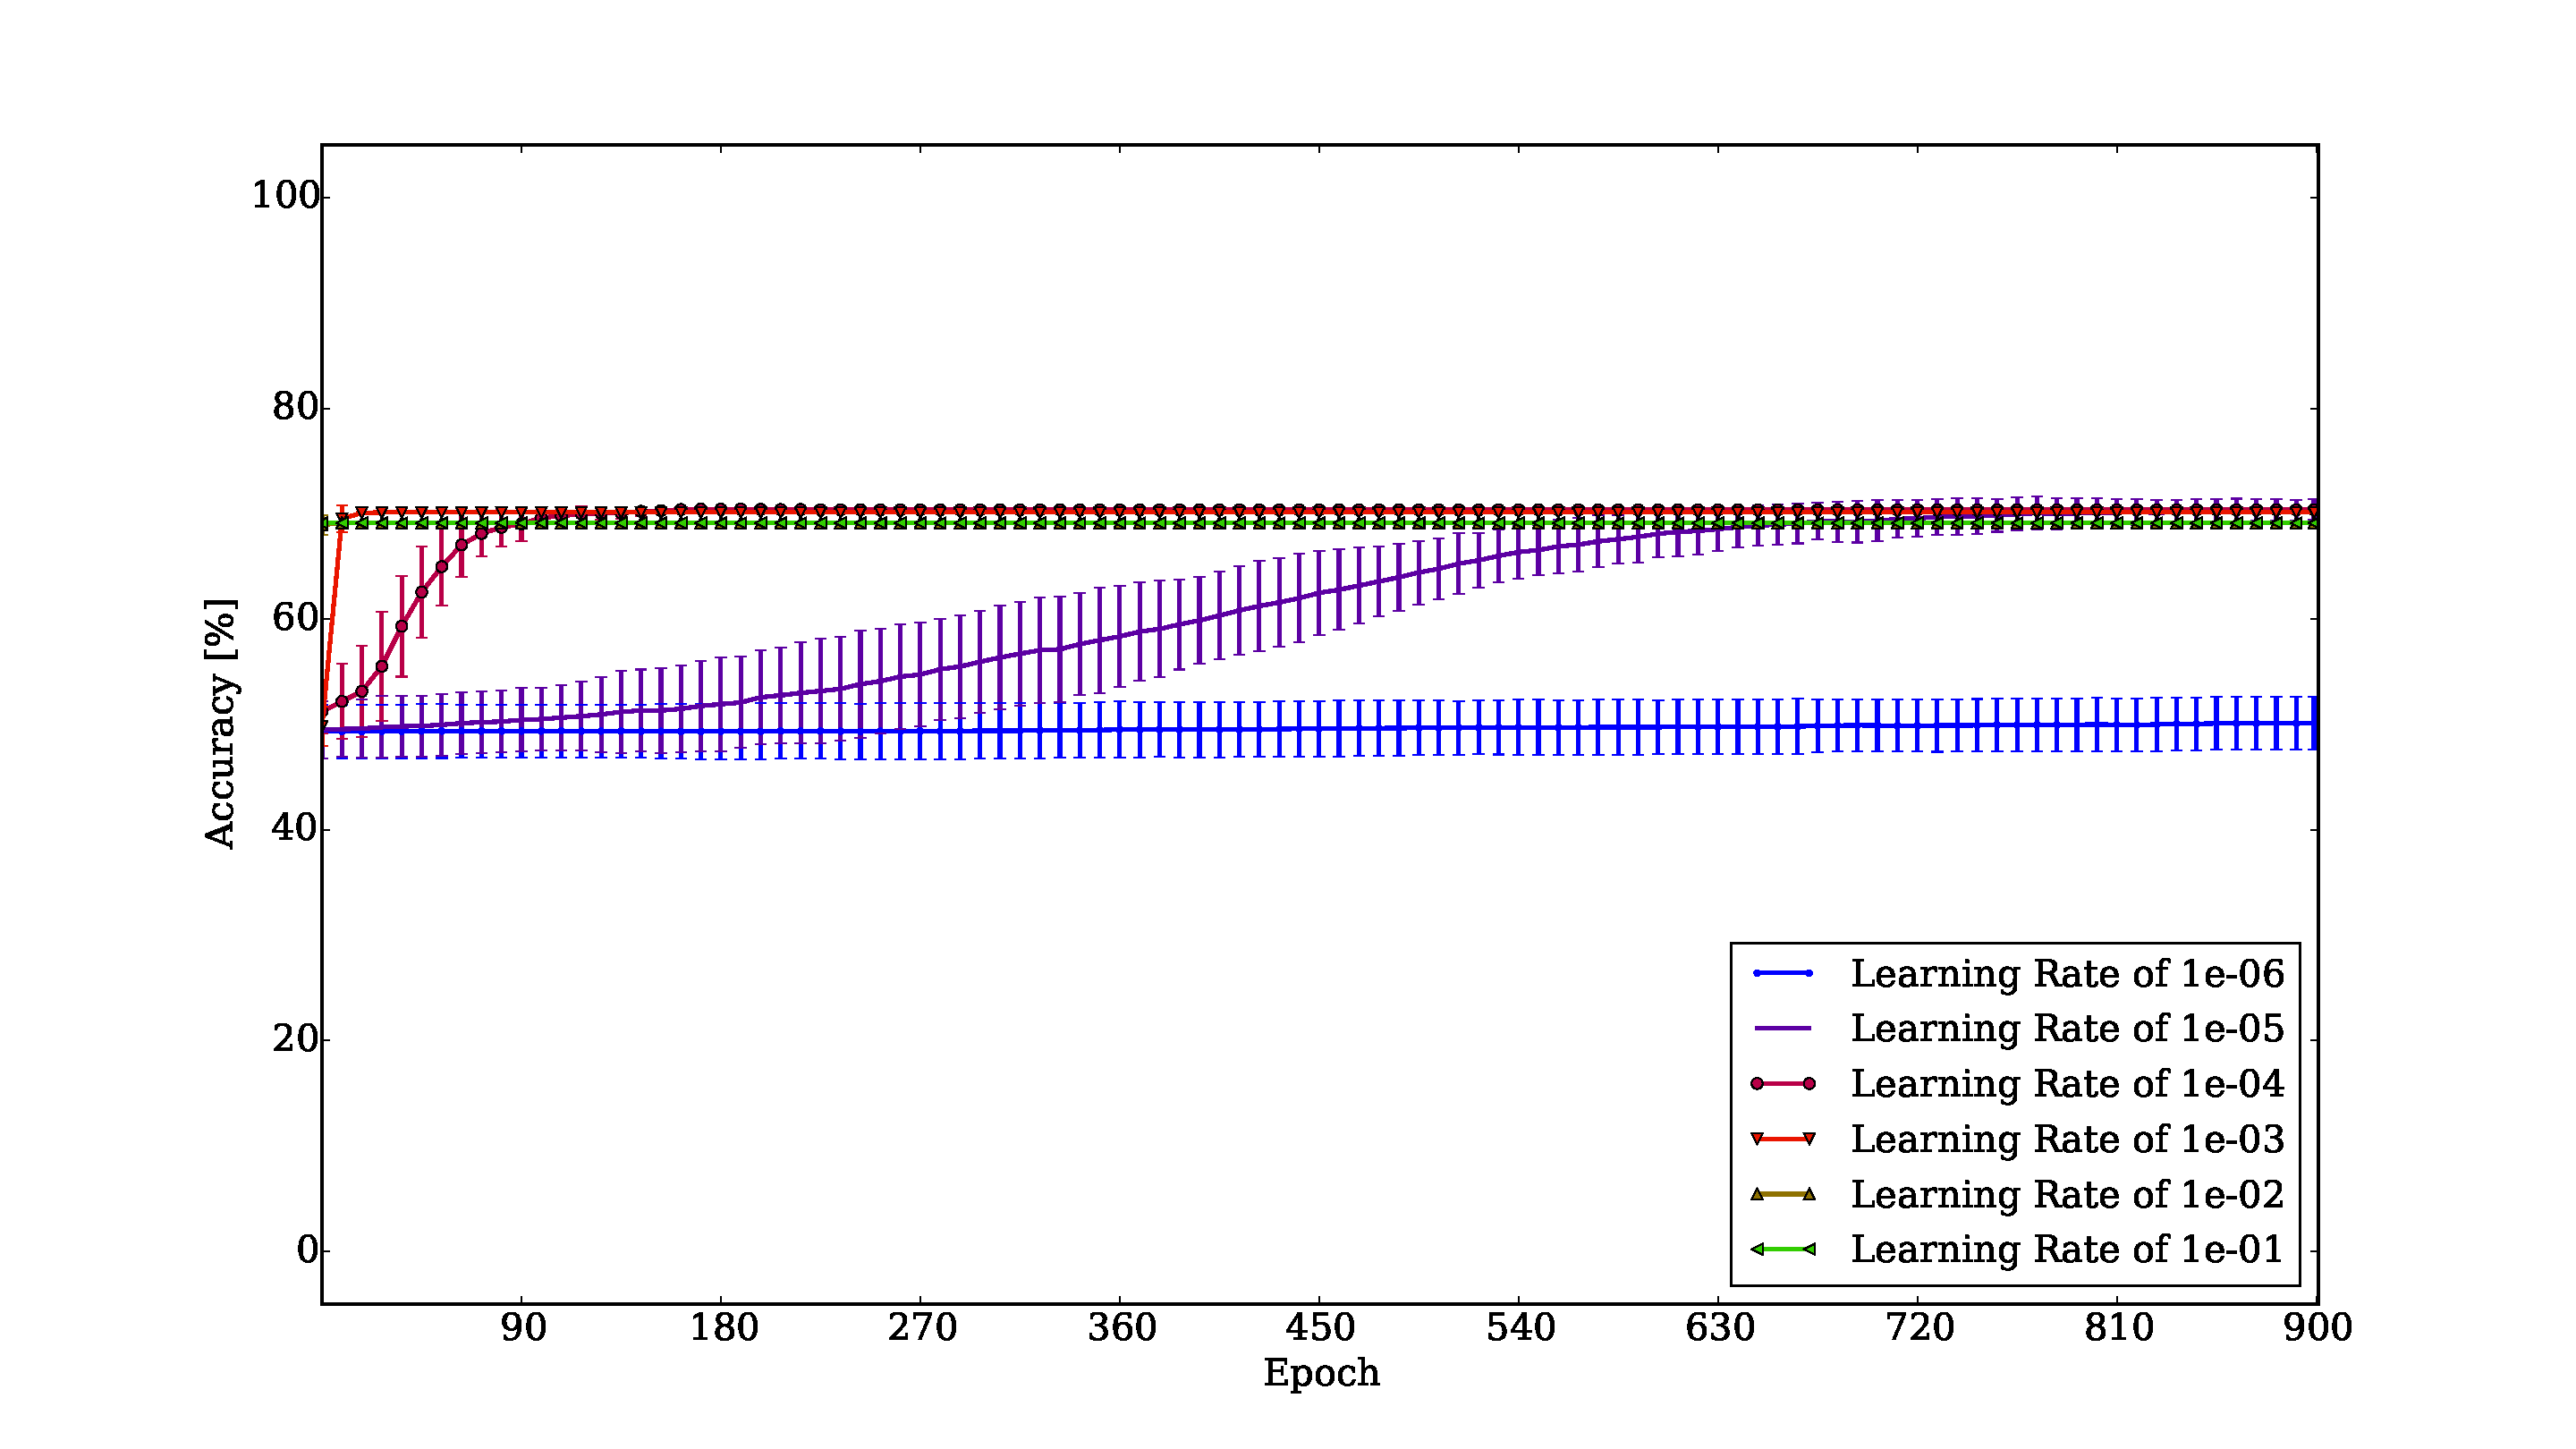
\includegraphics[width=0.49\linewidth]{sw_learning_rate_training}}
					\hfill
					\subcaptionbox
					{
						Testing results
						\label{fig:sw_learning_rate:testing}
					}
					{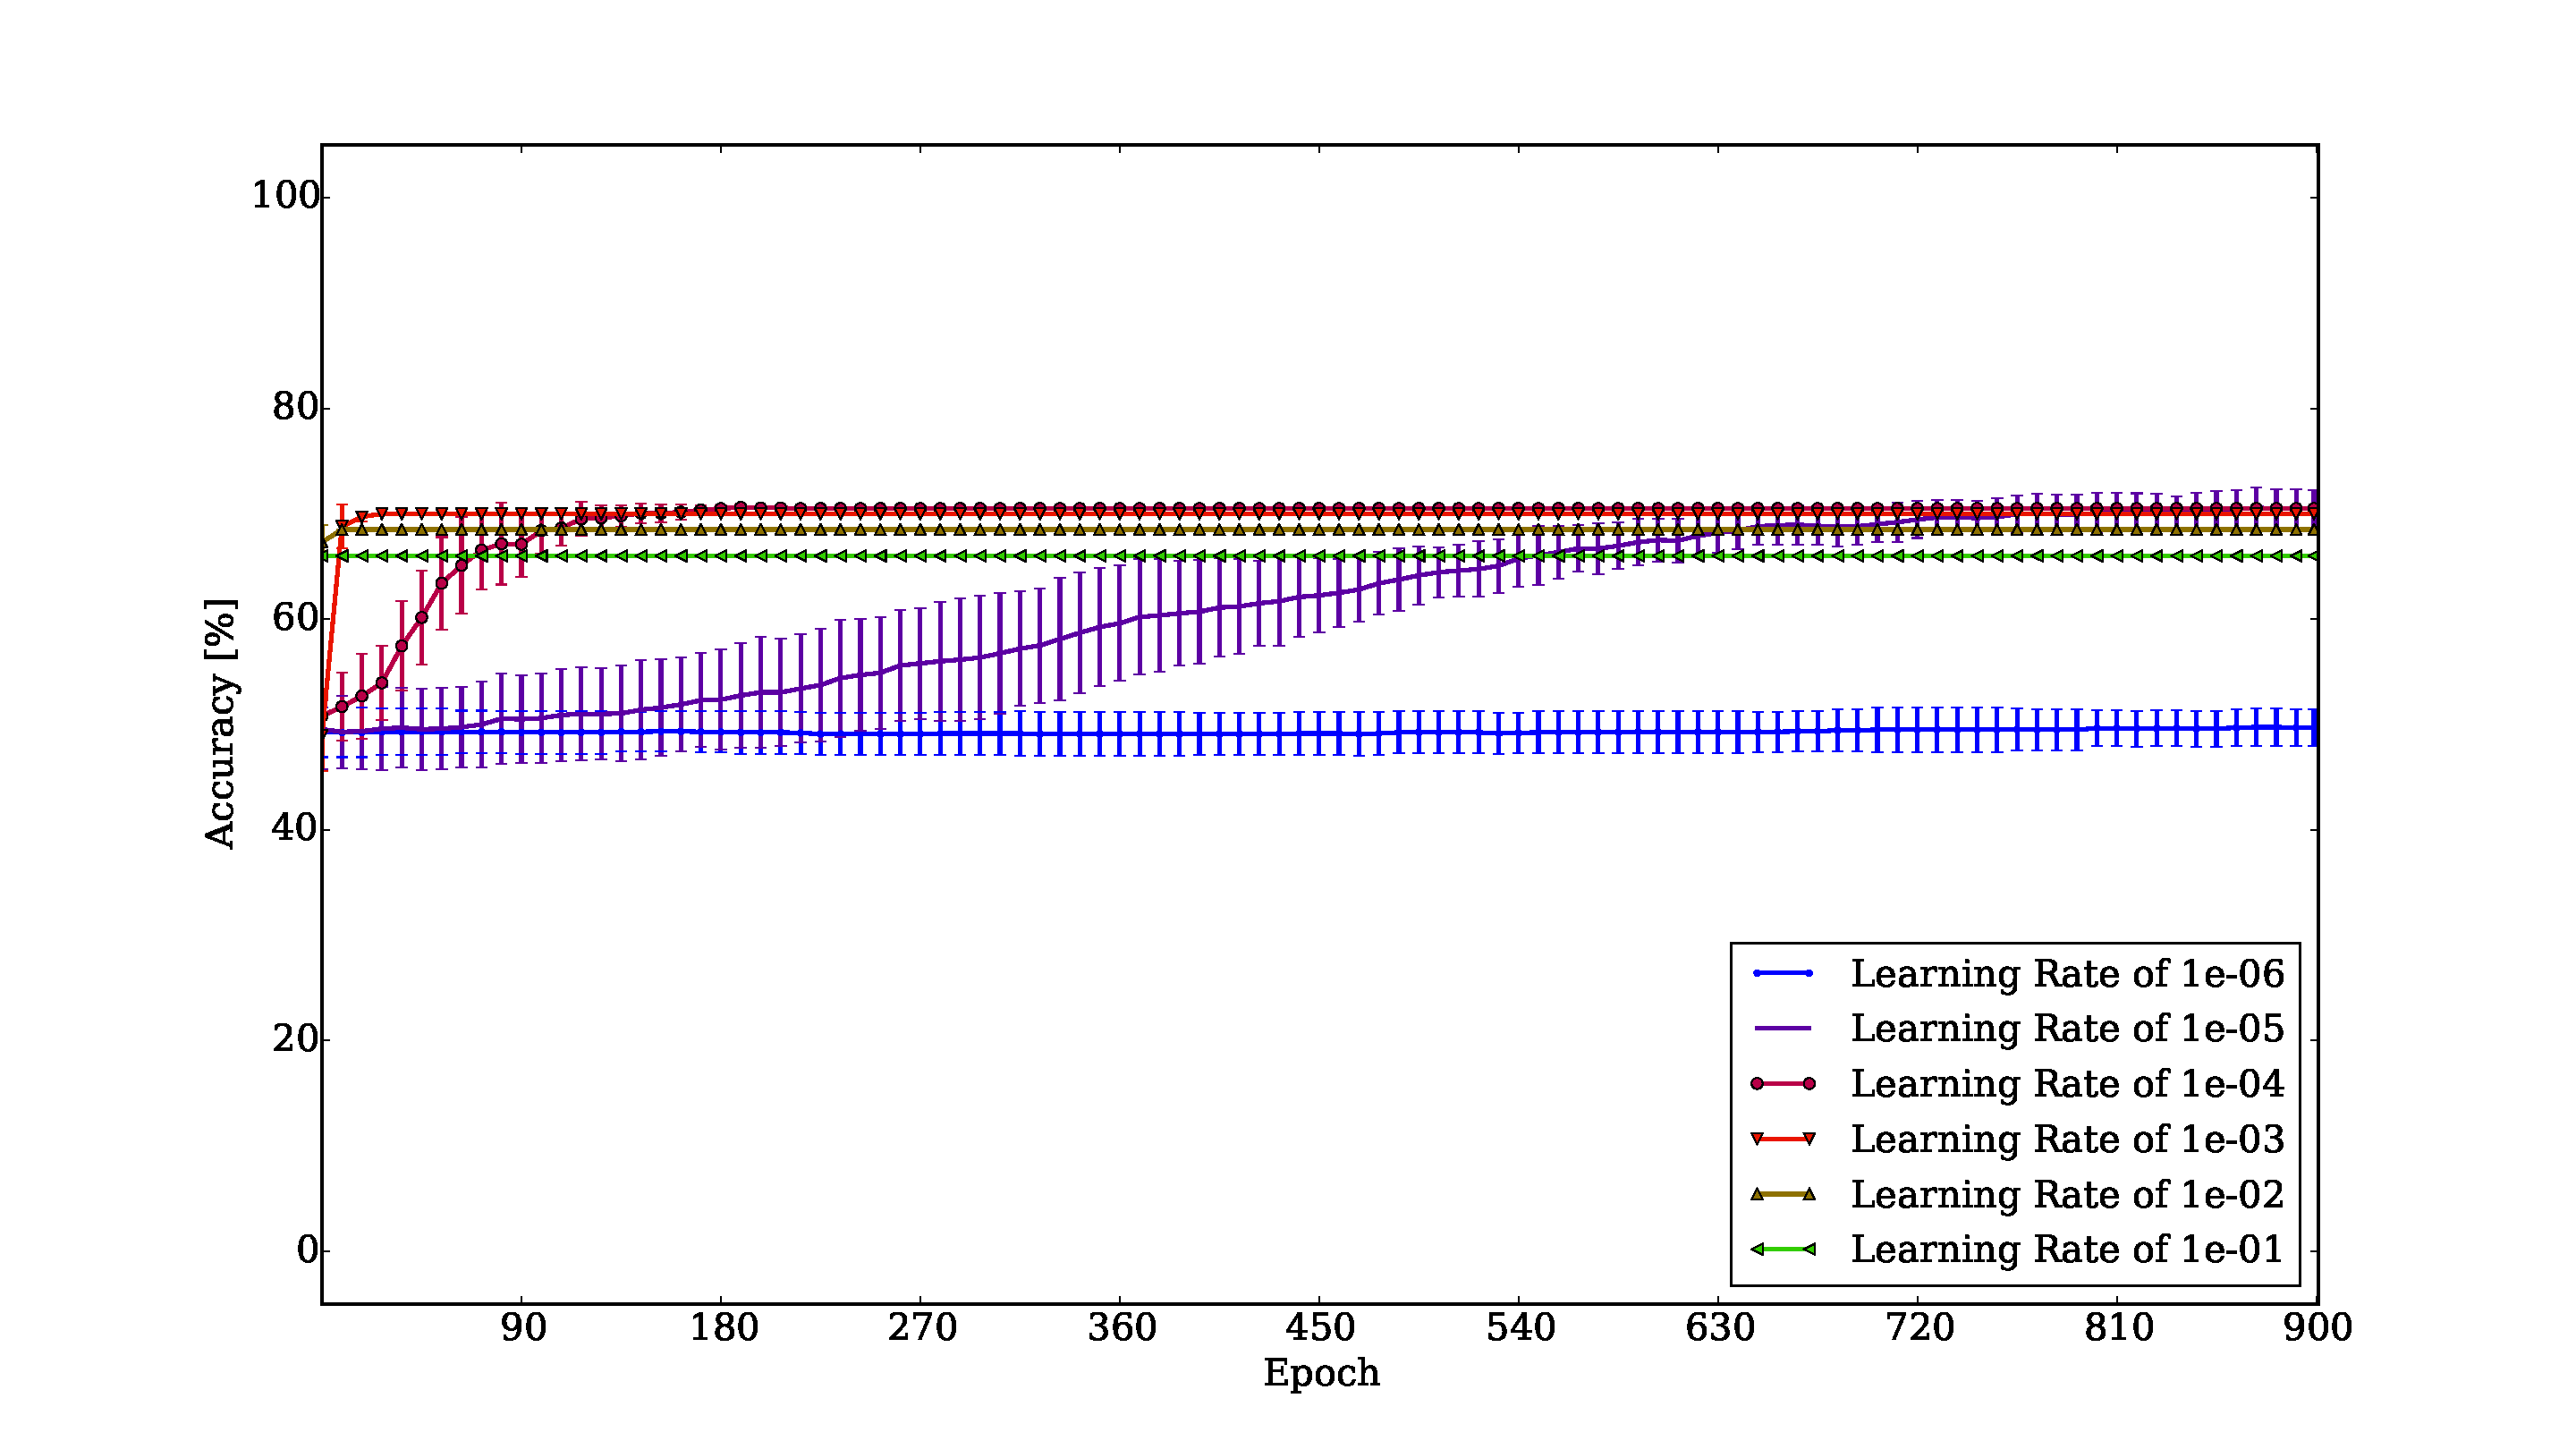
\includegraphics[width=0.49\linewidth]{sw_learning_rate_testing}}
					\hfill
					\caption{Training\subfig{fig:sw_learning_rate:training} and testing\subfig{fig:sw_learning_rate:testing} results for various learning rates. The image size was 7x7. Each network has a single output.}
					\label{fig:sw_learning_rate}
				\end{figure*}
				
				A fully generic software model of CLC was created in Python. This model supports \(I\) inputs, \(N\) networks, and \(O\) outputs. For gender classification only two networks are required (male and female); however, the number of inputs as well as outputs for each network can both be set to any suitable value. In addition to those parameters, a suitable learning rate had to be determined.
				
				To find suitable parameters, a simple search approach was taken, where one parameter was varied while all others were fixed. The best parameter from the current experiment was used in subsequent experiments. All simulations were performed 10 times for statistical purposes.
				
				The first parameter varied was the number of inputs, i.e. the image size. The number of outputs for each network was fixed at one and the learning rate was set to 0.001. The training and testing results are shown in \fig{fig:sw_img}. The full image size (30x30) produced the highest accuracy, as expected; however, an image size of 7x7 produced a similar level of accuracy and would reduce the number of inputs per network by over 18x. For this reason, an image size of 7x7 was chosen.
				
				The second parameter varied was the number of outputs. The image size was set to 7x7 and the learning rate was set to 0.001. The training and testing results are shown in \fig{fig:sw_outputs}. It is observed that a single output per network converges very quickly, while multiple outputs require hundreds of training epochs. Additionally, overfitting occurs once the number of epochs becomes too large. It is also observed that the variance increases drastically with multiple outputs. A final consideration is that once the number of outputs exceeds one, boosting must be performed. Boosting results in a substantial increase in HW complexity as it requires that a history of the past \(H\) outputs be stored per output. Additionally, an added computational strain is added for updating the boost values, calculating the network outputs, and selecting the network winner. For those reasons, a single output was chosen.
				
				The final varied parameter was the learning rate. The image size was set to 7x7 and the number of outputs for each network was fixed at one. The training and testing results are shown in \fig{fig:sw_learning_rate}. When the learning rate is within a suitable range, the system converges on a similar output. If the learning rate is too small, the system is unable to learn. If the learning rate is too high, the system is unable to expand upon its learning. A learning rate of 0.001 was chosen, as this resulted in the best accuracies with the fastest convergence. This learning rate is additionally within a range suitable for representation within hardware.
			
			\paragraph{Hardware Model}
				\begin{figure*}[t!]
					\captionsetup[subfigure]{position=b}
					\centering
					\hfill
					\subcaptionbox
					{
						Training results
						\label{fig:sw_fractional_bits:training}
					}
					{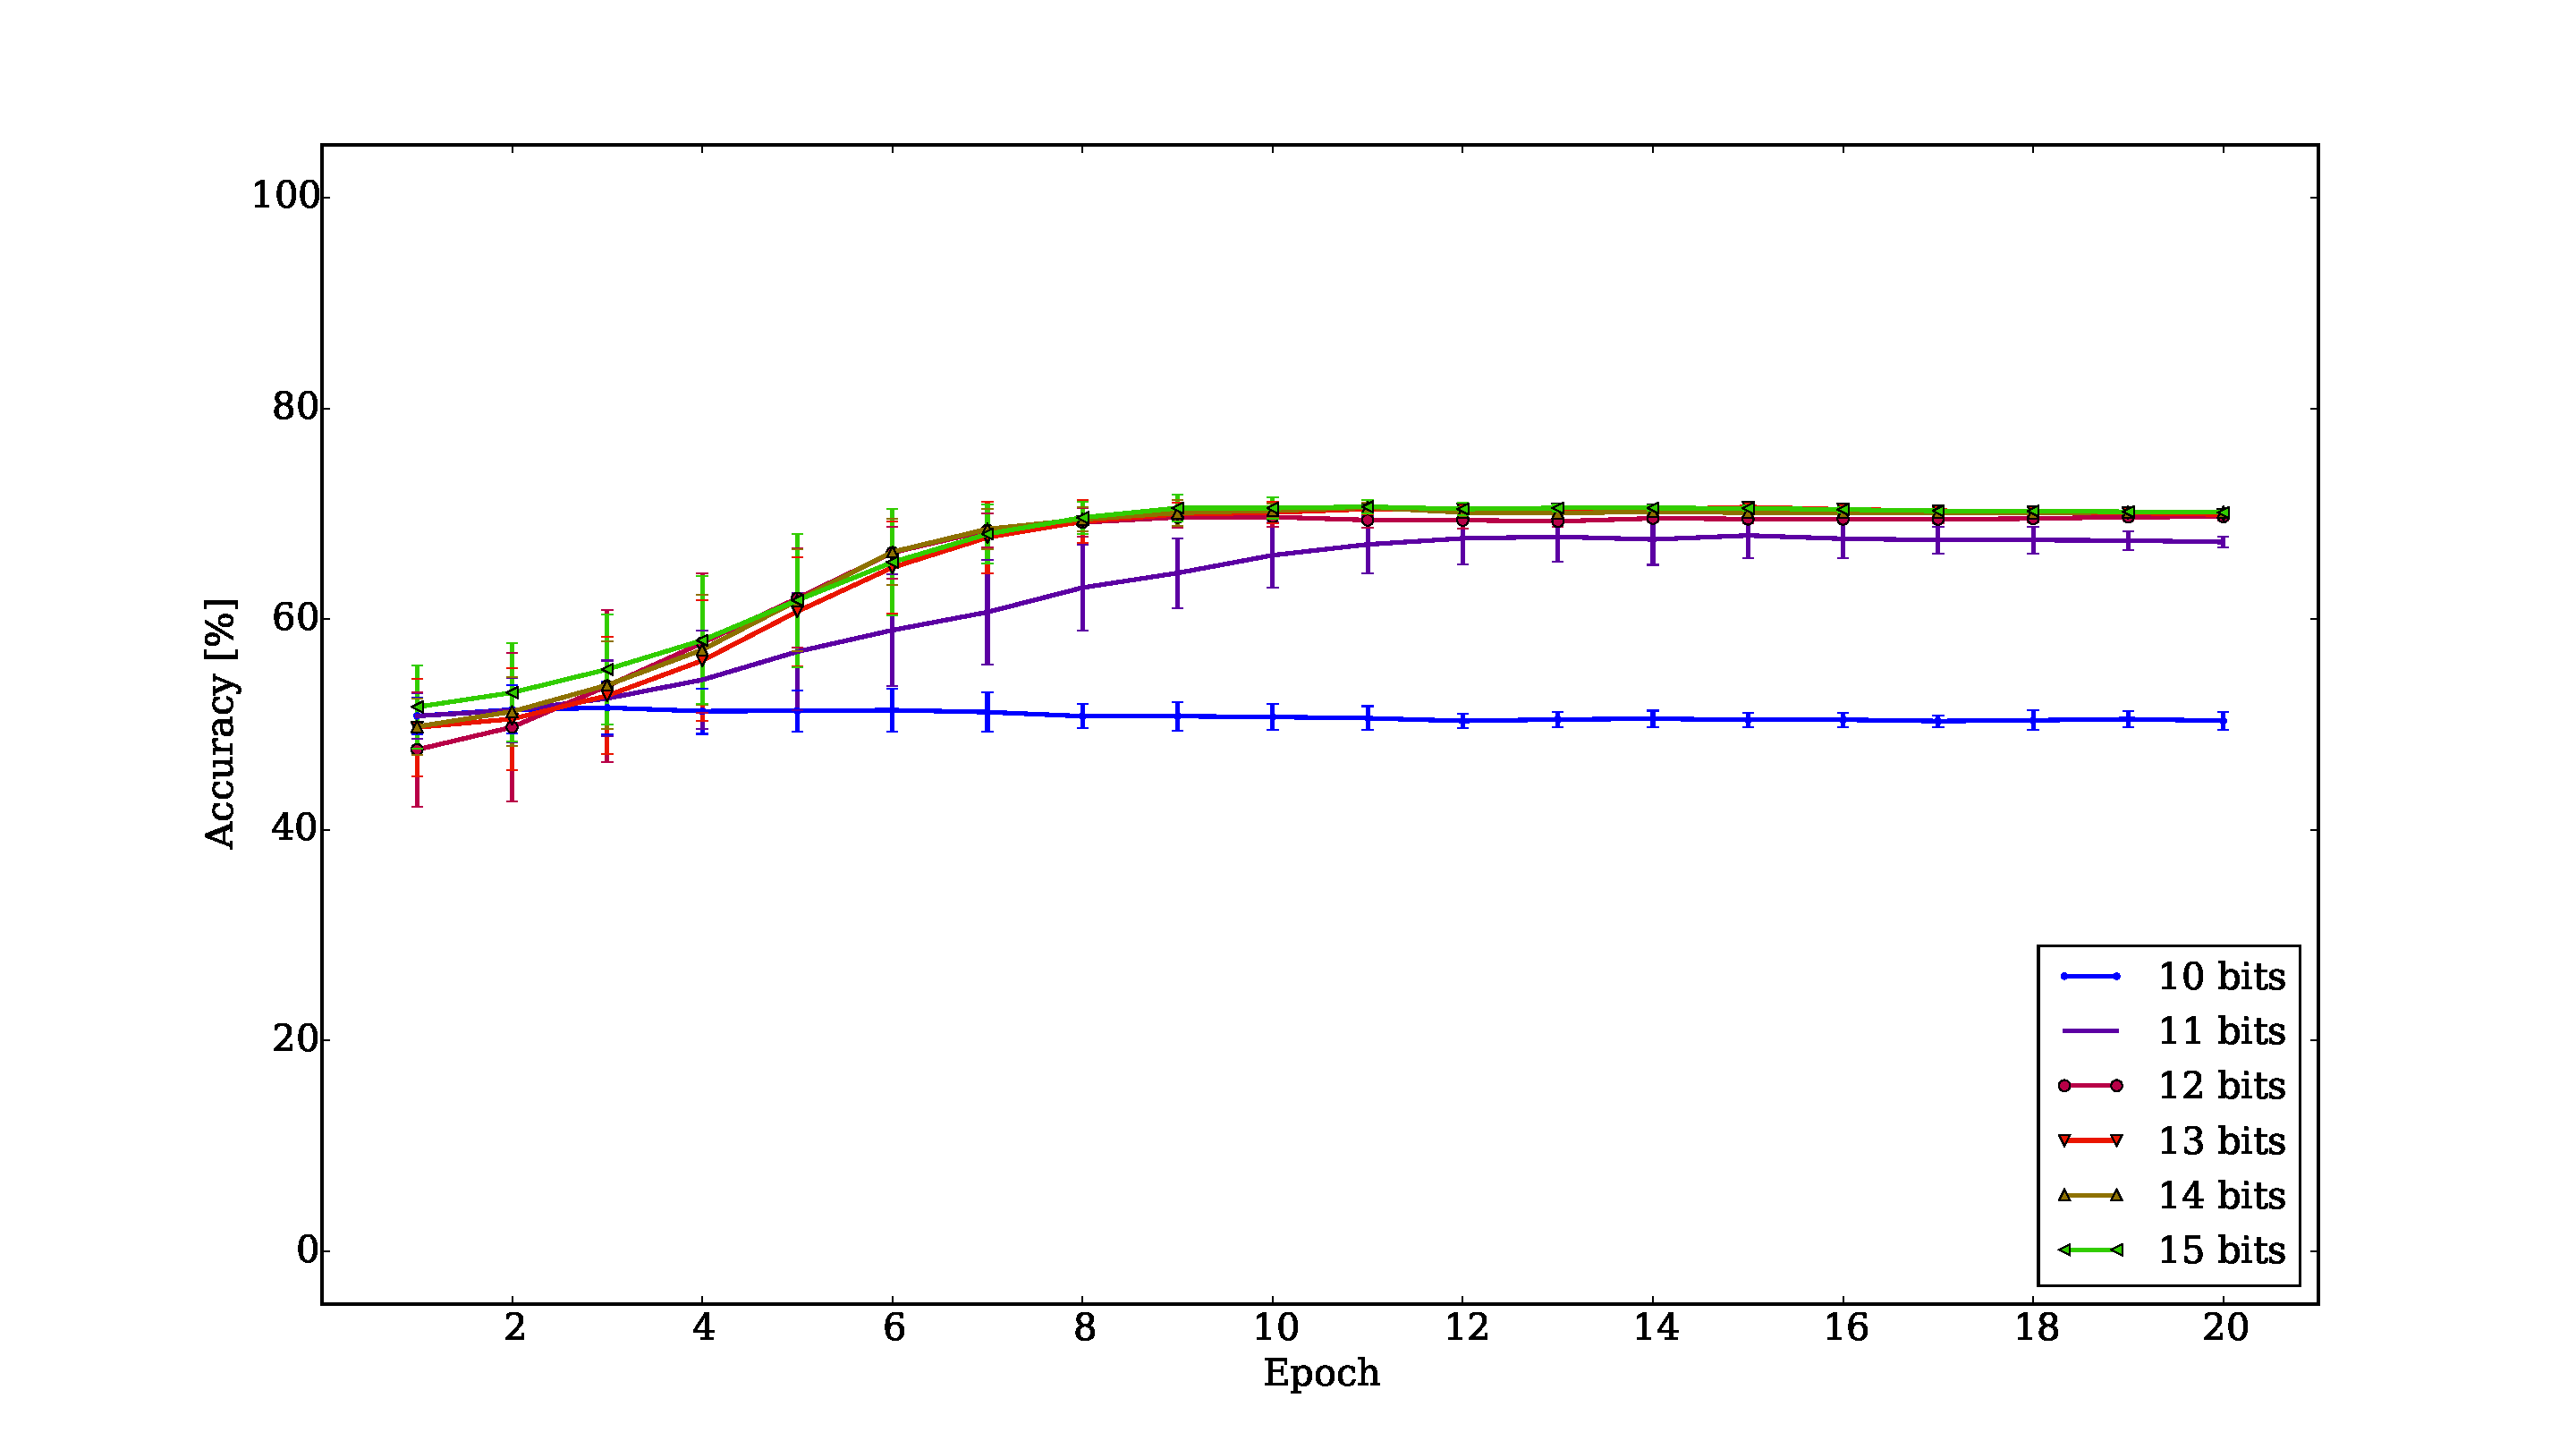
\includegraphics[width=0.49\linewidth]{sw_fractional_bits_training}}
					\hfill
					\subcaptionbox
					{
						Testing results
						\label{fig:sw_fractional_bits:testing}
					}
					{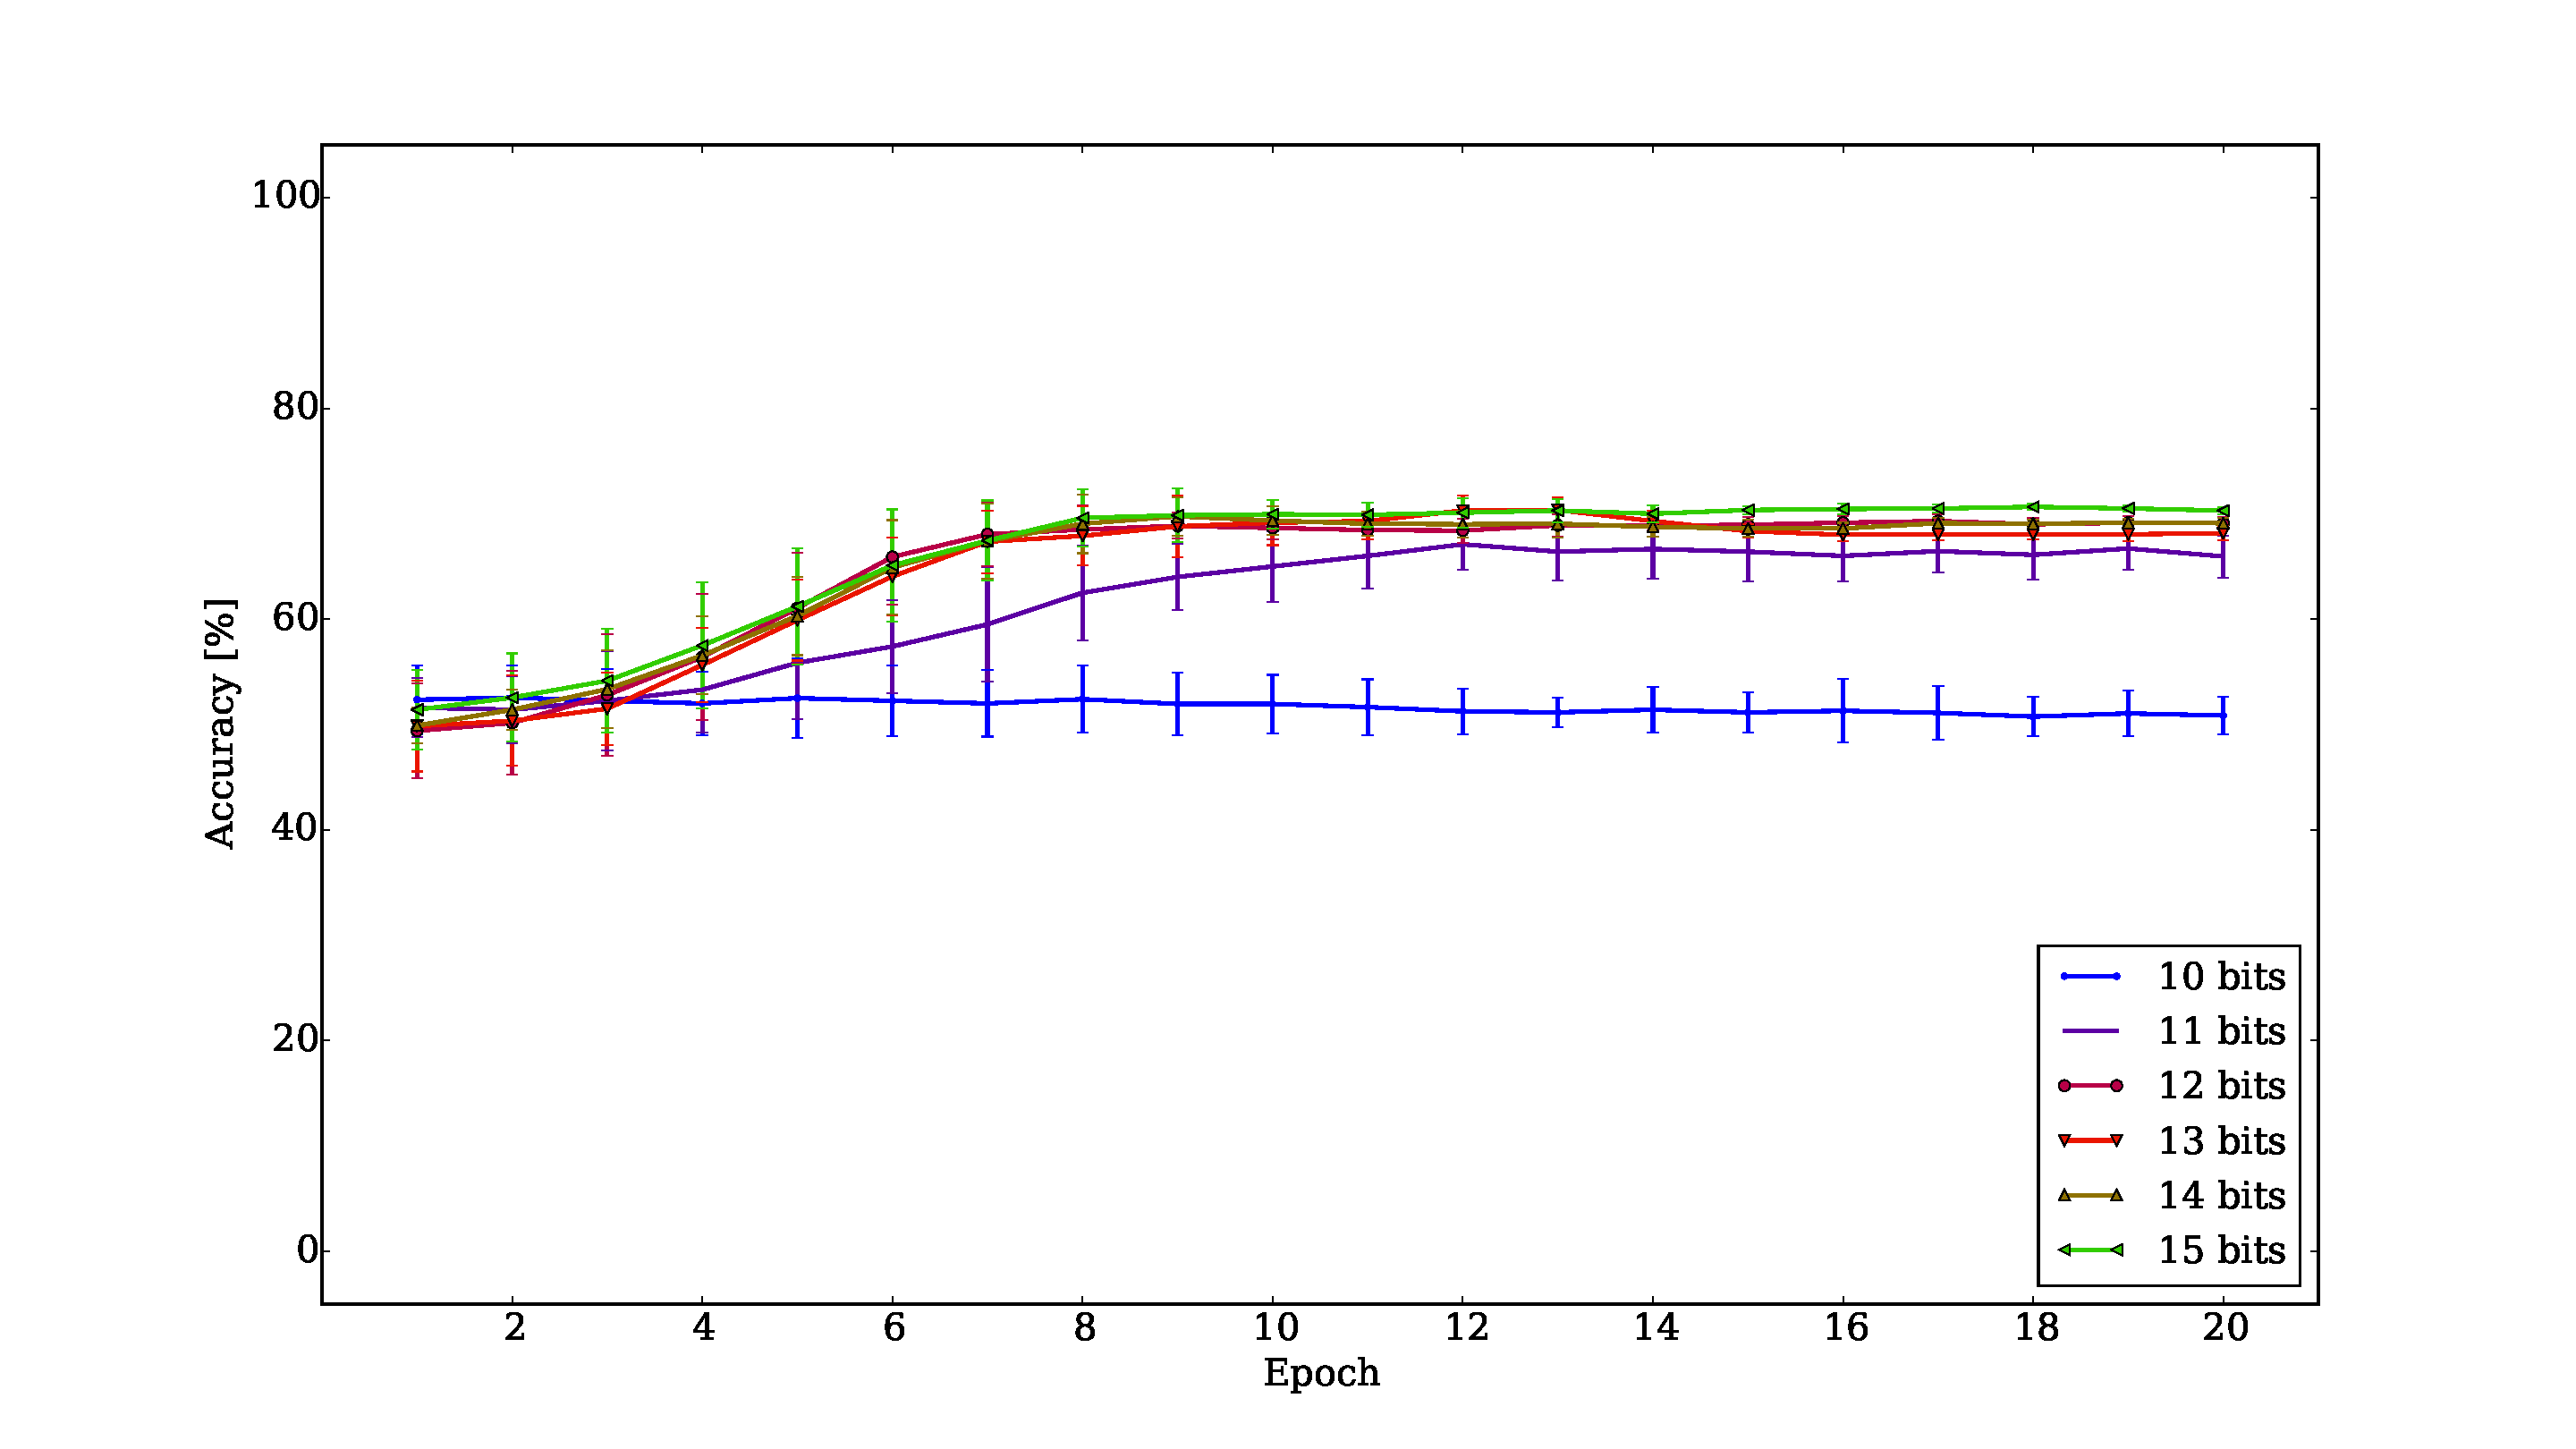
\includegraphics[width=0.49\linewidth]{sw_fractional_bits_testing}}
					\hfill
					\caption{Training\subfig{fig:sw_fractional_bits:training} and testing\subfig{fig:sw_fractional_bits:testing} results for a various count of fractional bits.}
					\label{fig:fractional_bits}
				\end{figure*}
				
				The CLC model was redesigned to follow the hardware model as closely as possible. Boosting was removed from the model as it was assumed that there would only be a single output from each network. It was desired to use the Q fixed-point number format for representing all numbers. A Python datatype was created to allow all required arithmetic operations to be performed as a native Python datatype. This allowed for multiple benefits, namely ensuring that the arithmetic would resolve to the same exact values as in the hardware (including overflow and underflow conditions) and allowing for a near seamless transition between the pure software model and this new model.
				
				In Q format it is important to know exactly what the bounds of the scalars will be. If they grow to be too large or too small, then they will no longer be able to be represented with the specified number of integer bits. Additionally, the level of precision must be noted. Each increase in decimal precision requires more fractional bits. With these concepts in mind, it is important to ensure that the numbers are all at a similar scale, as this will reduce the number of required bits. The chosen learning rate is 0.001, which is a relatively small number, and the magnitude of the weights and pixels are between zero and one. To keep the number of bits down, it was desired to ensure that the values did not exceed \(\pm{1}\), because only a single integer bit would be required.
				
				In \eq{sw_weight_update}, \(\hat{y}_{o,n}^{(p)}\) is always going to be equal to one, as there is only a single network output and this output must always be chosen to be the winning cluster. The difference of \(u_i^{(p)}\) and \(w_{i,n}\) is able to be between -2 and 2, so with a single integer bit it is possible to have overflow; however, it is an unlikely scenario and should not drastically affect the overall output, as an overflow would result in the max positive value being returned. More importantly, because both \(u_i^{(p)}\) and \(w_{i,n}\) are of the same scale, the operation will result in a similar returned scale. This value is then going to be scaled by \(\alpha\), reducing the resulting scale to be the same as \(\alpha\)'s. Since \(I < \alpha^{-1}\) it is not possible for the resulting weight to overflow. This allows for \eq{sw_weight_update} to be simply updated to \eq{hw_weight_update}.
				
				In \eq{sw_output}, the squared values of the difference of \(u_i^{(p)}\) and \(w_{i,n}\) are being summed. Squaring that difference will occur in an overflow in many cases. Additionally, summing those squared values will almost certainly result in an overflow. To address that problem, \eq{sw_output} is updated to be \eq{hw_output}, where \(C\) is a scaling factor defined to be \(I^{-1/2}\). This scaling factor ensures that the sum remains within a suitable range; additionally, performing the scaling operation before squaring eliminates overflow from that operation.
				
				\begin{equation}
					\label{hw_weight_update}
					\Delta w_{i,n} = \alpha(u_i^{(p)}-w_{i,n})
				\end{equation}
				
				\begin{equation}
					\label{hw_output}
					\hat{y}_{o,n}^{(p)} = \displaystyle\sum_{i=1}^{I}((w_{i,n} - u_i^{(p)})*C)^2
				\end{equation}
				
				This hardware model introduces another parameter, the number of suitable fractional bits. To determine the minimum number of required bits, this new model was simulated across a range of count of fractional bits. The training and testing results are shown in \fig{fig:fractional_bits}. As seen, once the number of fractional bits drops below 11 the system is no longer able to function. At 11 bits or above, the accuracies are similar, thus 11 bits were chosen. This results in a total of 13 bits per number, which is still much smaller than the number of bits that would be required if floating point had been used.
		
		\subsubsection{Hardware}
			The hardware implementation (\fig{fig:System:block}) was designed to be identical to the software implementation. The system was designed structurally (\fig{fig:full:system}), allowing for modularity as well as flexibility in optimization. The system was divided into three main parts: two calculation blocks (one for the weight update during training and one for the output evaluation during testing) and a register block (used for storing the weights). These main components are controlled by a state machine.
			
			\begin{figure}[t]
				\captionsetup[subfigure]{position=b}
				\centering
				\hfill
				\subcaptionbox
				{
					Entity
					\label{fig:System:block}
				}
				{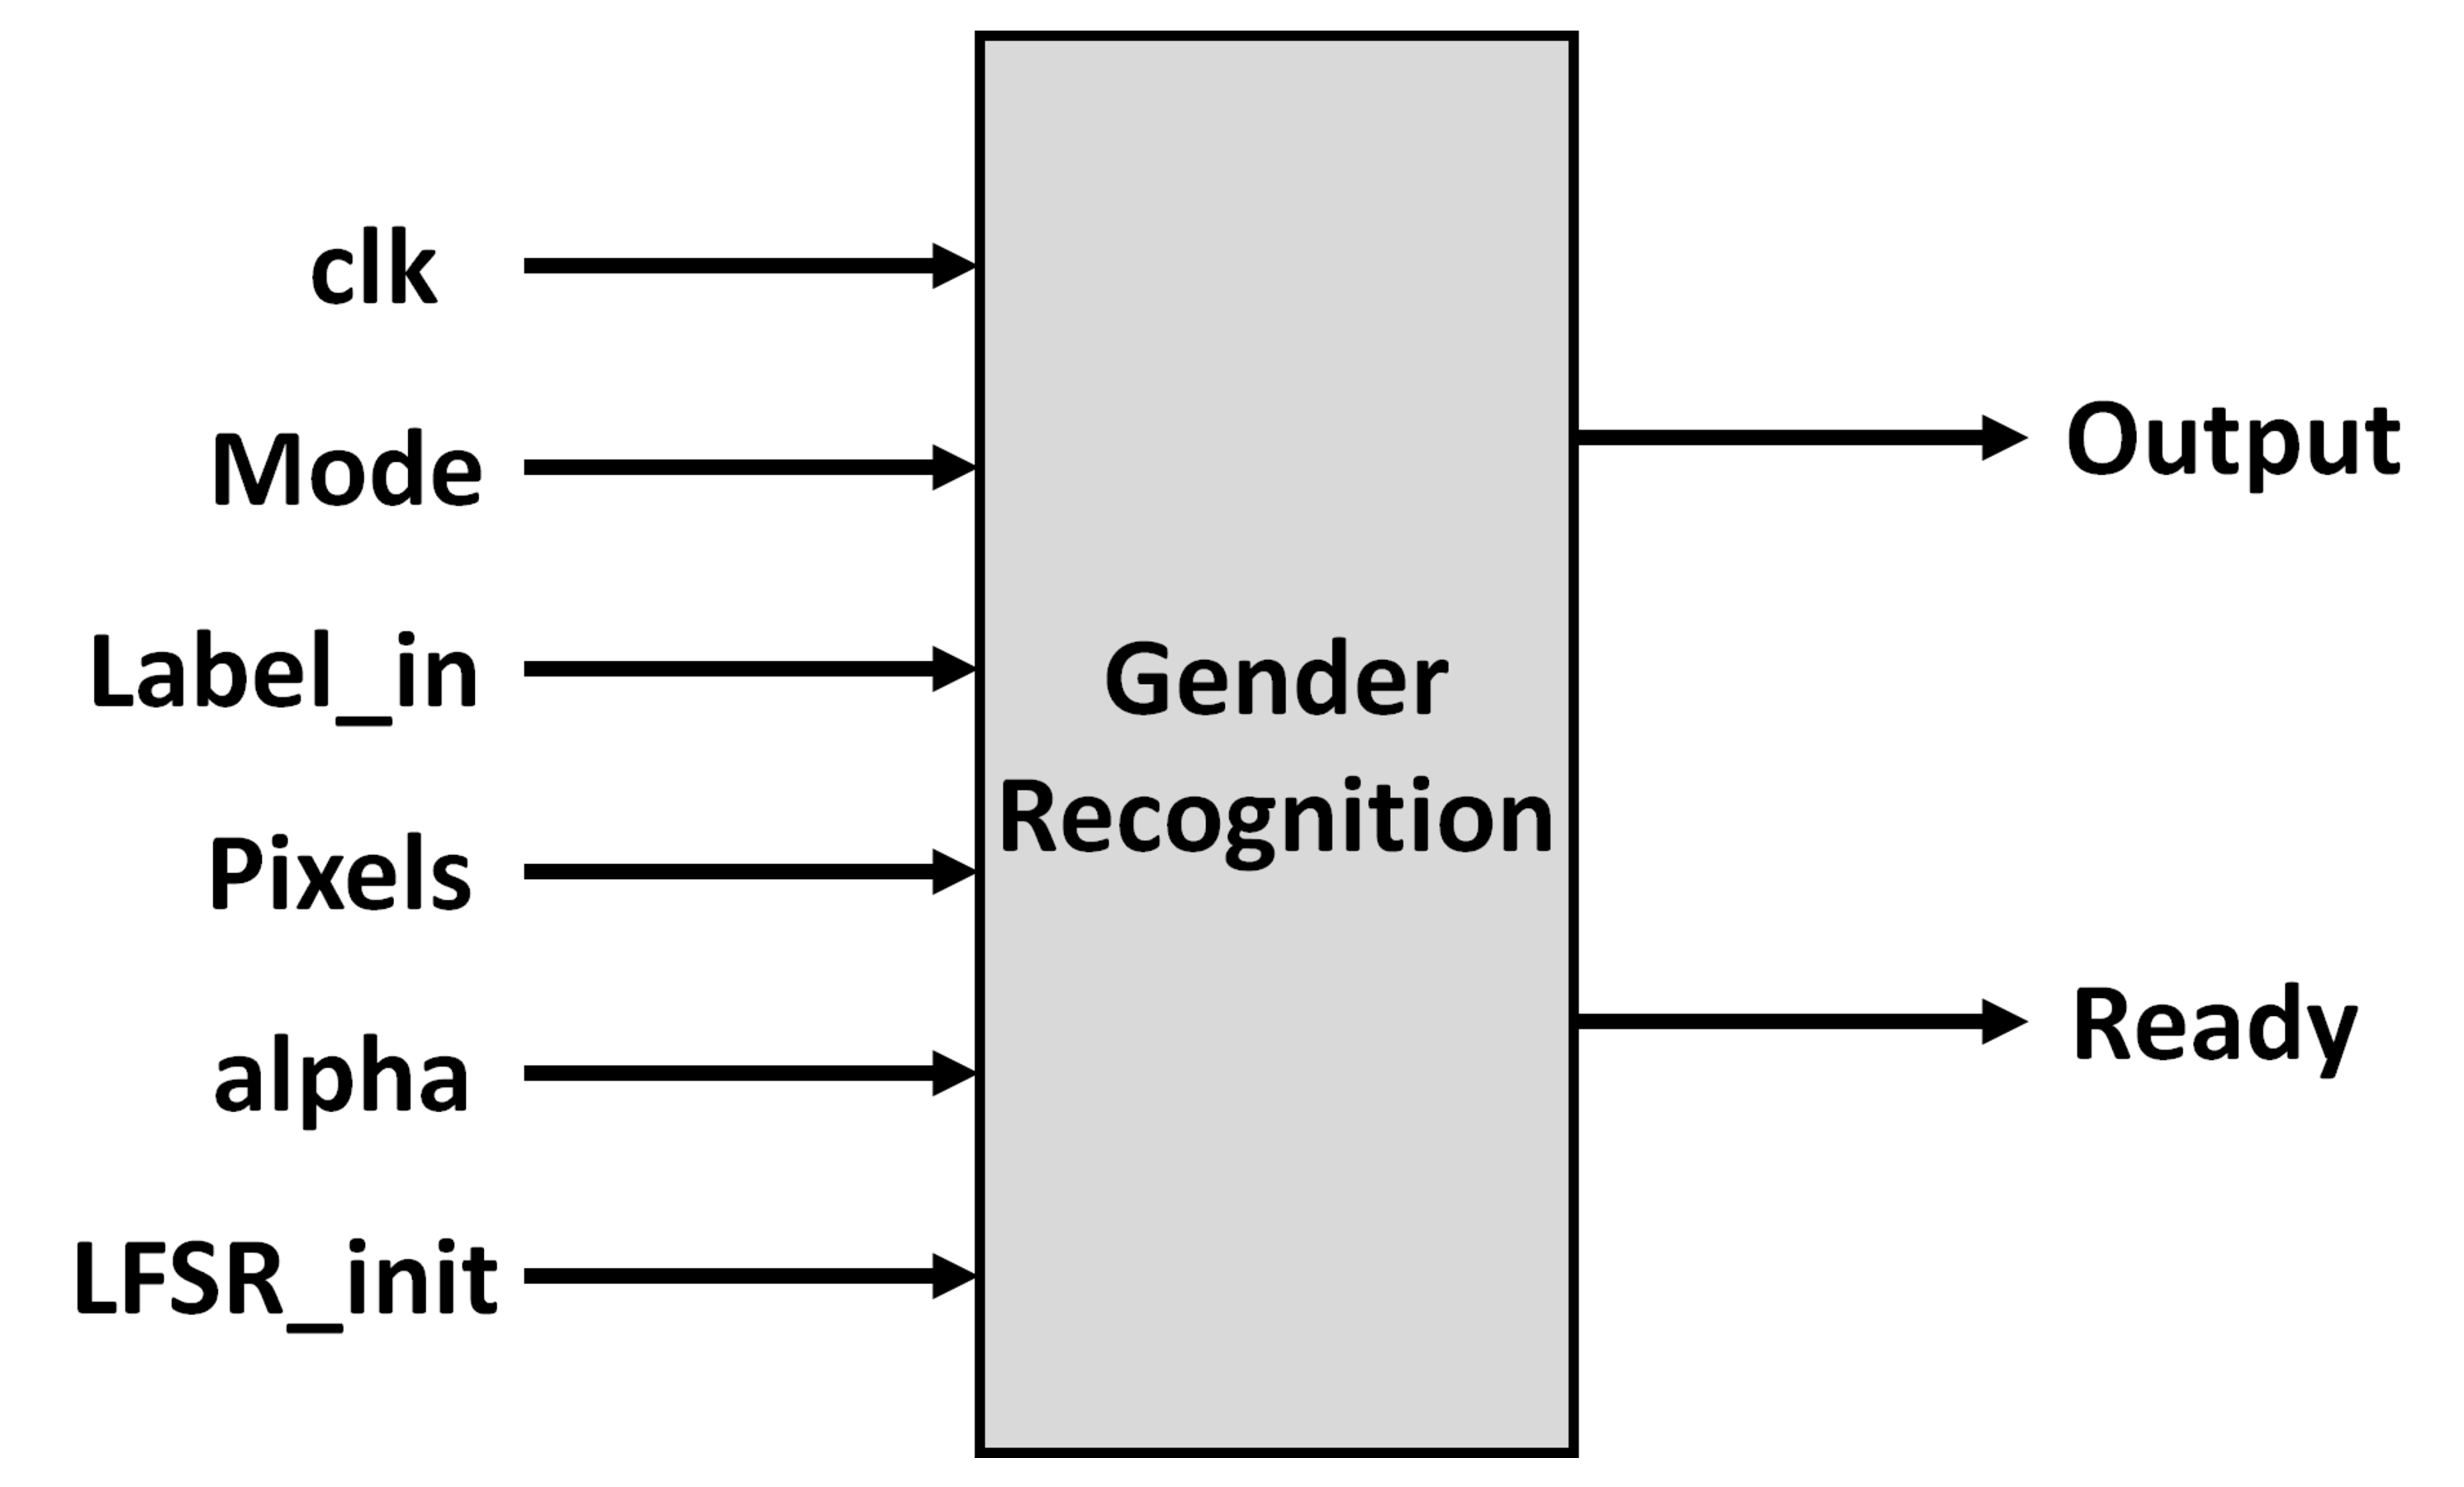
\includegraphics[width=0.9\columnwidth]{System_block}}
				\hfill
				\subcaptionbox
				{
					Internal structure
					\label{fig:full:system}
				}
				{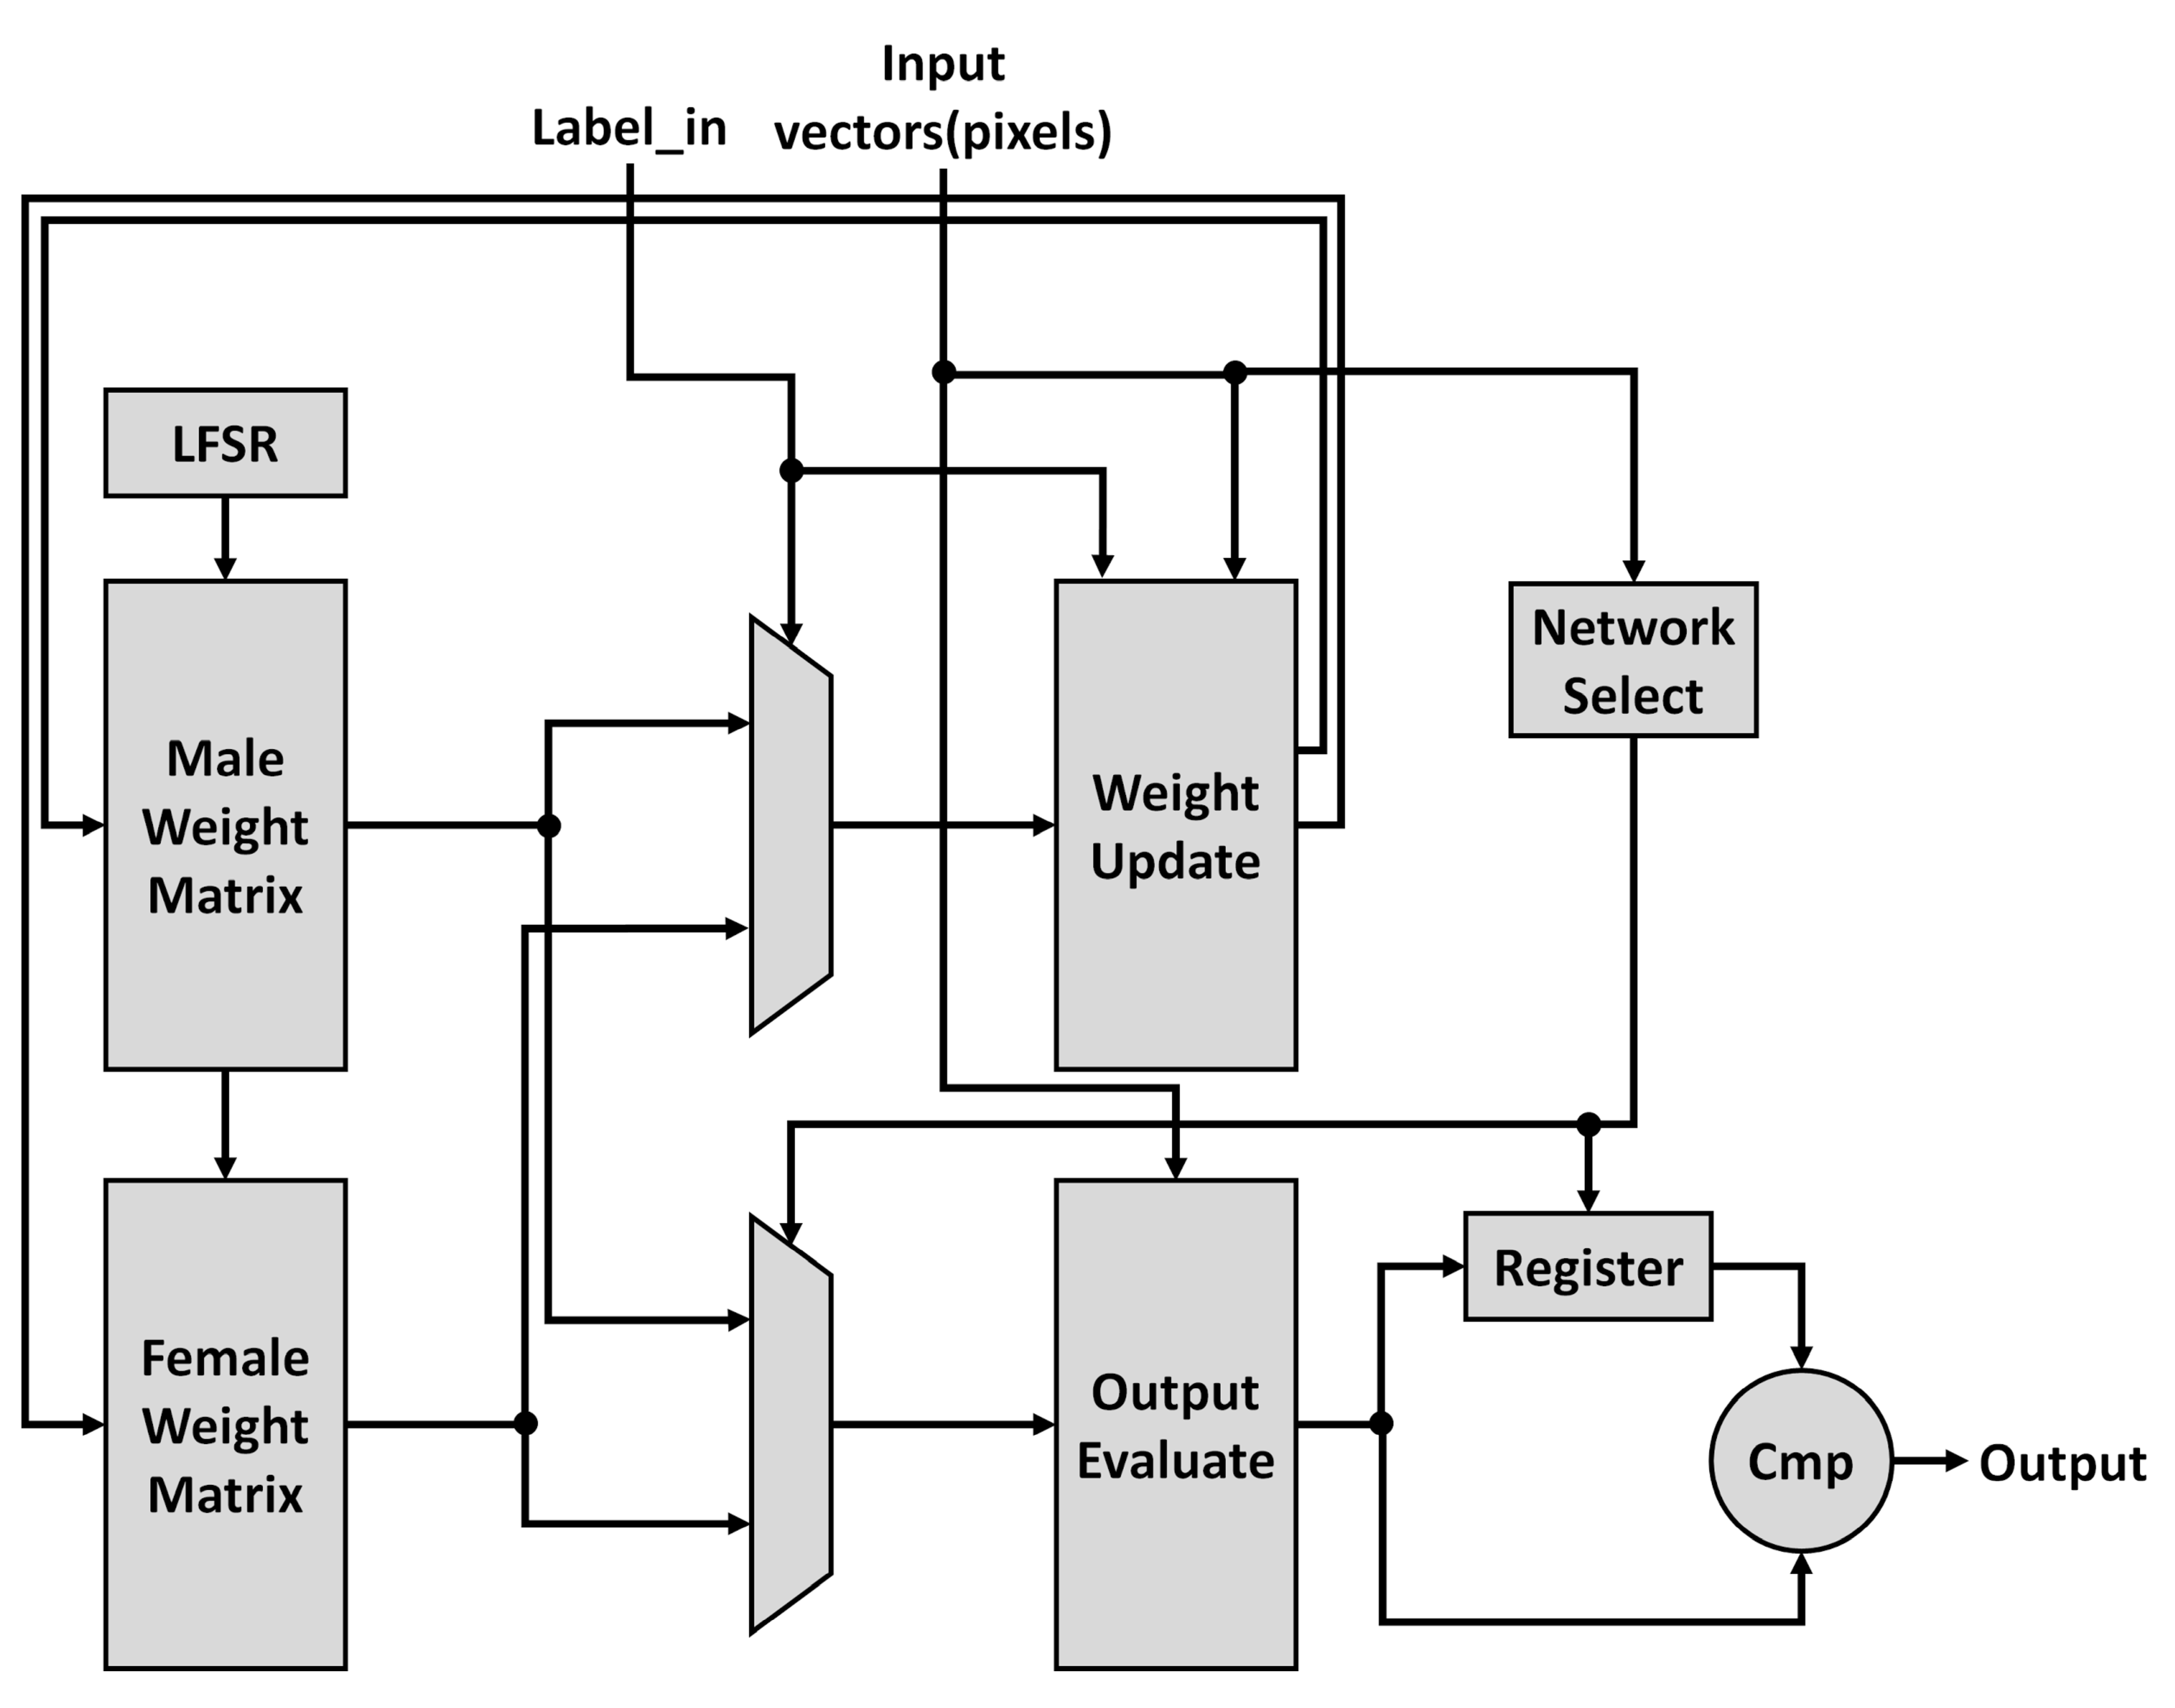
\includegraphics[width=0.9\columnwidth]{Full_system}}
				\hfill
				\caption{System block\subfig{fig:System:block} showing the hardware entity and the internal structure of the hardware\subfig{fig:full:system} showing the main components of the system: weight registers, weight update, output evaluate, LFSR, and comparator.}
				\label{fig:hardware:system}
			\end{figure}
			
			The state machine, shown in \fig{fig:state:machine}, is the main control unit of the system. The input signal, \textit{Mode}, controls the transition between the following states: \textit{Idle}, \textit{Initialization}, \textit{Training}, and \textit{Testing}. Based on those states the statuses of the output flags are changed. One external and three internal flags are driven by the state machine. The external flag is \textit{Ready}. The internal flags are \textit{Test}, \textit{Train}, and \textit{Reset}. Those flags are used to control the system. The system starts in \textit{Idle} and waits for any changes in \textit{Mode}. From \textit{Idle} the state machine transits to all other states. The default use of the system is to transition to \textit{Idle} between all other states.
			
			\begin{figure}
				\centering
				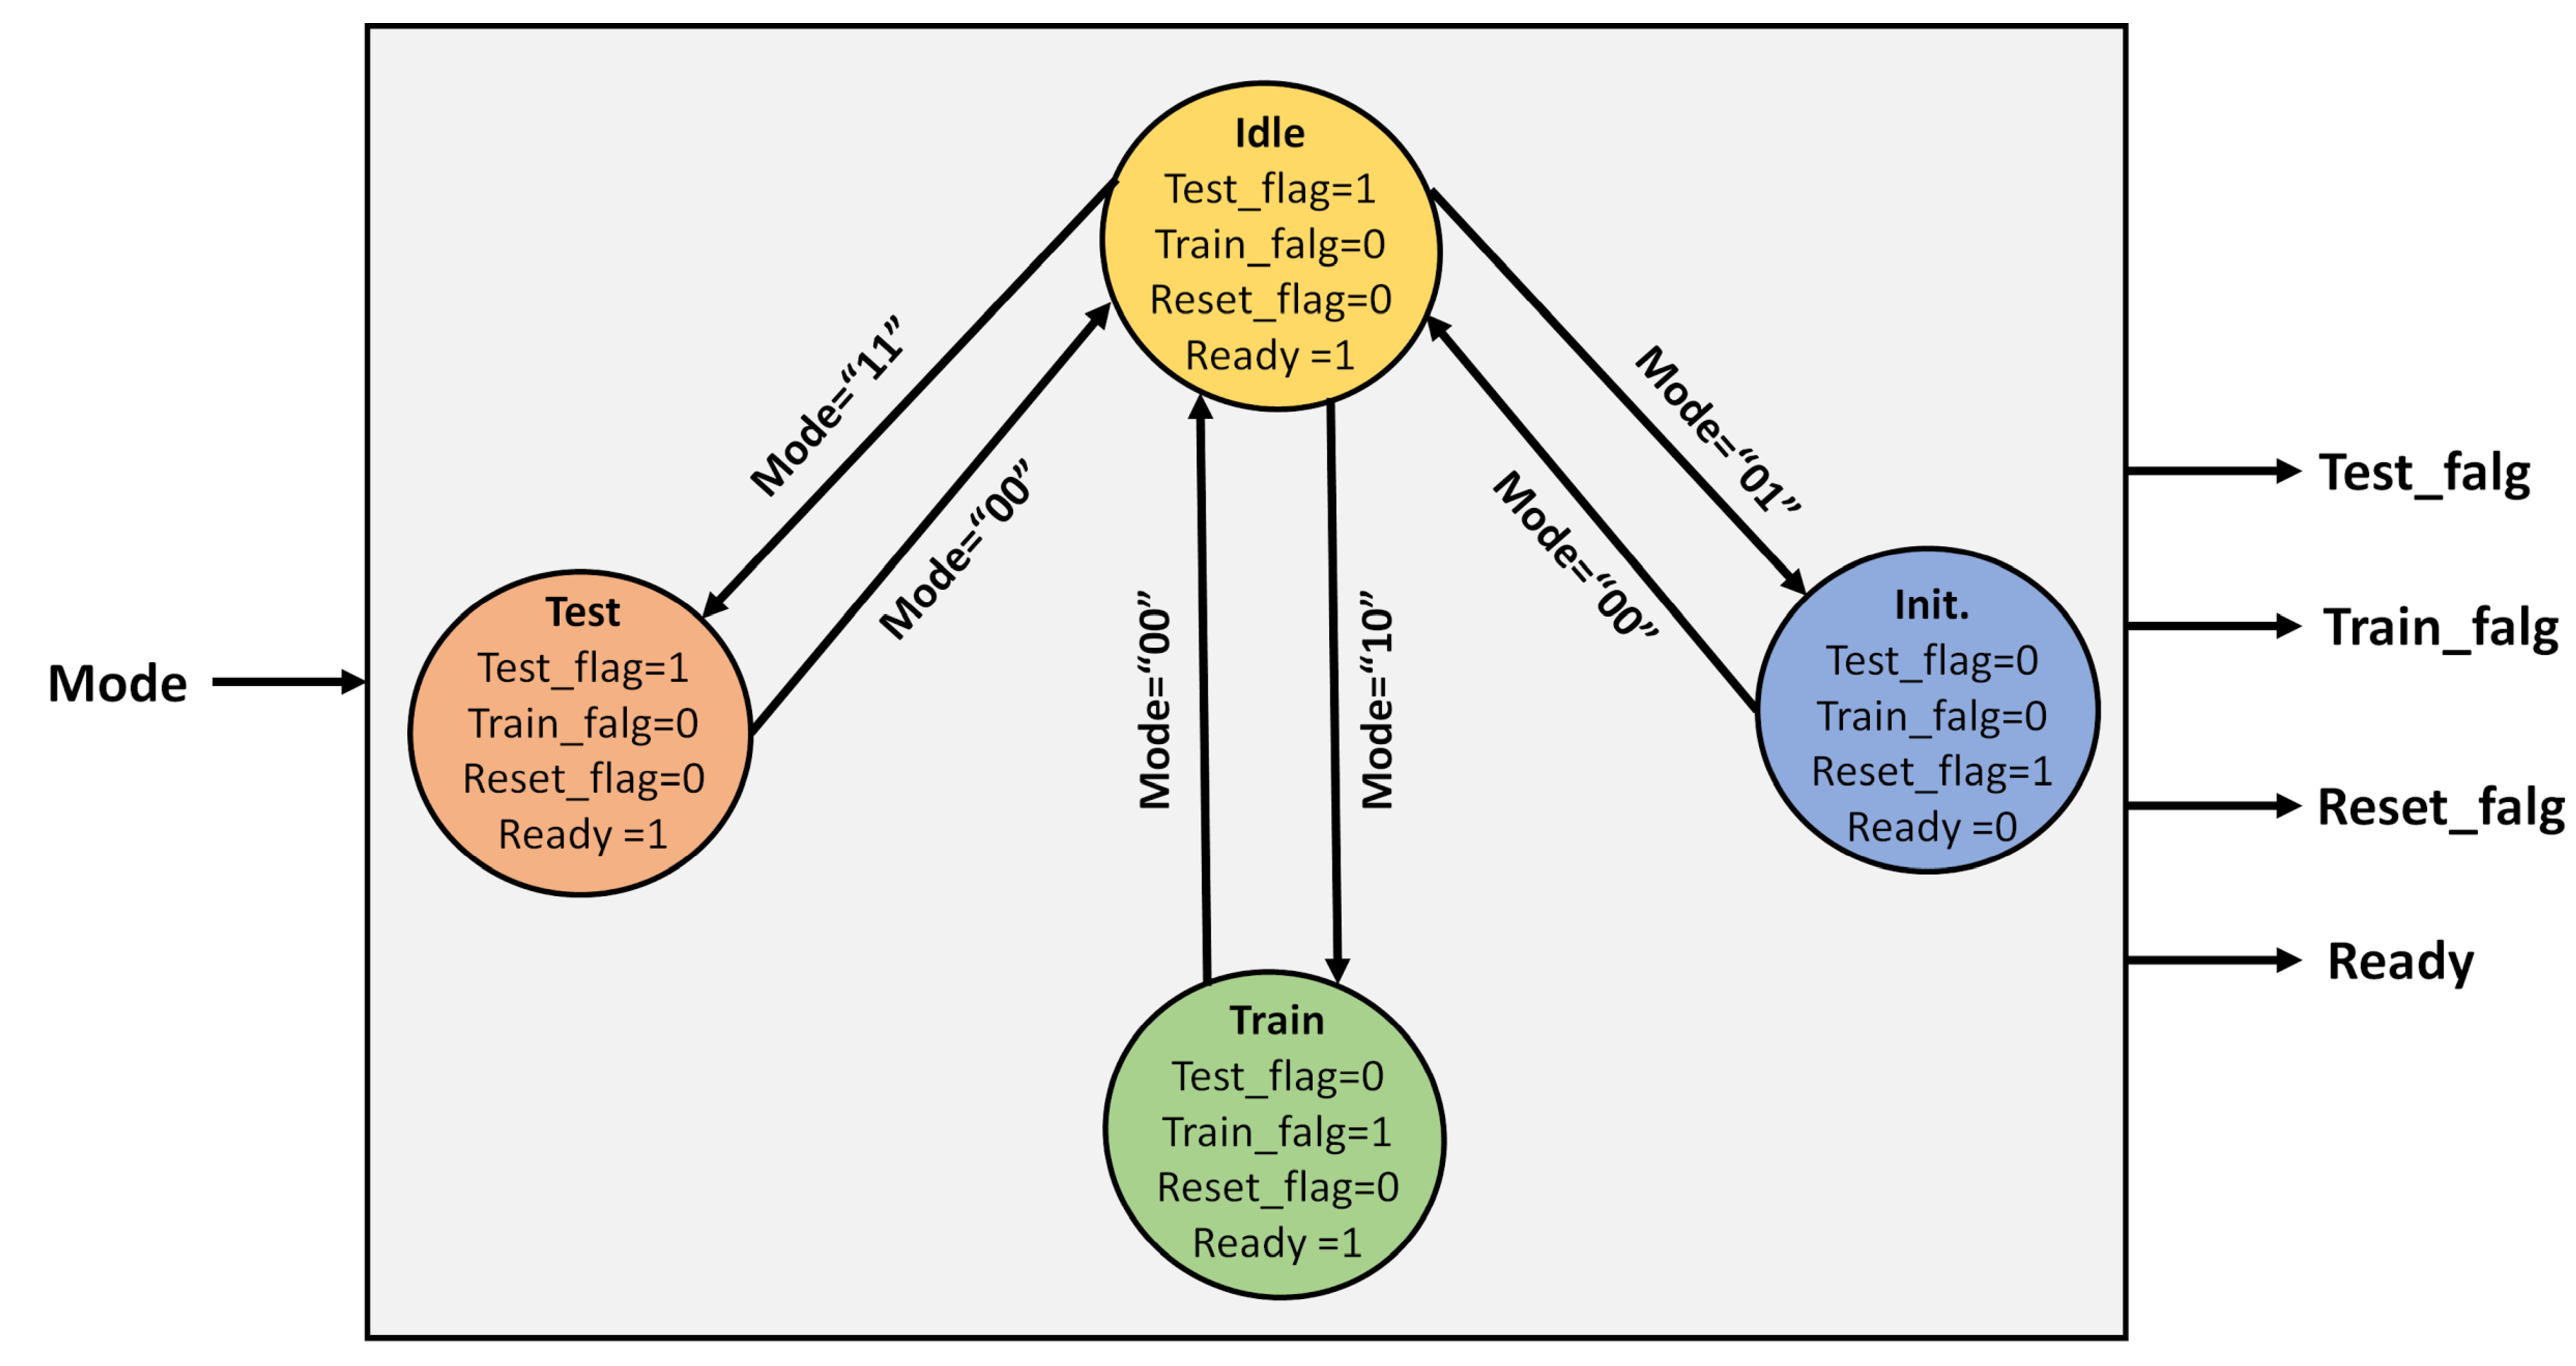
\includegraphics[width=0.8\linewidth]{State_machine}
				\caption{State machine consisting of one input \textit{Mode} and four ouputs. \textit{Mode} controls the transition between the states (\textit{Idle}, \textit{Initialization}, \textit{Training}, and \textit{Testing}). The four output flags control the internal operation of the system.}
				\label{fig:state:machine}
			\end{figure}
			
			During \textit{Initialization} the weights are randomly generated and stored in the male and female weight register banks. A 12-bit Linear Feedback Shift Register (LFSR) is used to generate the initial weights. The configuration of the LFSR is shown in \fig{fig:lfsr}. Once the reset flag is active, the LFSR component takes the seed value from the input port \textit{LFSR\_init}. From that seed it generates the initial weight values at a rate of one value per clock cycle. Those values are then serially fed into the male and female weight register banks.
			
			During \textit{Training} the weights are updated by the weight update block. Each weight update takes two clock cycles. In the first clock cycle the appropriate weight block (male or female) sets its weights to be active. The weight update block takes the assigned weights and calculates the updated weights based on the input image. In the second clock cycle the new weight update values are saved into the associated weight's registers. The weight update block consists of a stack of identical smaller components. Each component is responsible for updating one weight value, as defined by \eq{hw_weight_update}. The internal structure of one weight update component is shown in \fig{fig:weight:update}, where \(\alpha\) is the learning rate as defined by the port \textit{alpha}.
			
			There is no limit on the number of training vectors that the system can learn. The user can supply new vectors as long as the system is in the \textit{Training} state. Once the training process is completed, \textit{Mode} should be set back to \textit{Idle}. Returning back to \textit{Idle} ensures that the training process will gracefully complete.
			
			During \textit{Testing} the output evaluate block (\fig{fig:output:evaluate}) is used to calculate the output value of the network, as defined by \eq{hw_output}. This block consists of a stack of one pixel's output evaluate component followed by an adder tree. The adder tree performs the summation of the individual weight-input distance calculations. The scale factor used in this component is saved in a register located in the output evaluate block and is distributed to all components in the block. This block is able to compute the output of a network every clock cycle.
			
			\begin{figure}[t]
				\captionsetup[subfigure]{position=b}
				\centering
				\hfill
				\subcaptionbox
				{
					LFSR
					\label{fig:lfsr}
				}
				{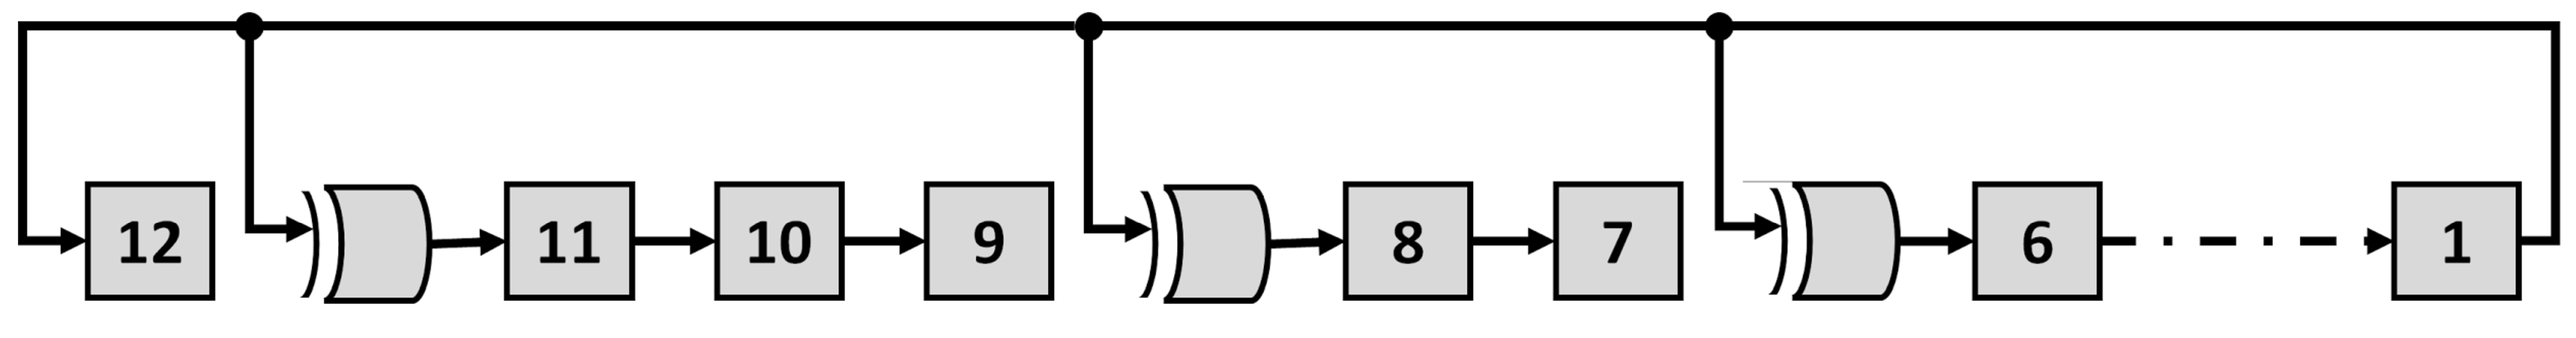
\includegraphics[width=0.9\columnwidth]{LFSR}}
				\hfill
				\subcaptionbox
				{
					Weight update component
					\label{fig:weight:update}
				}
				{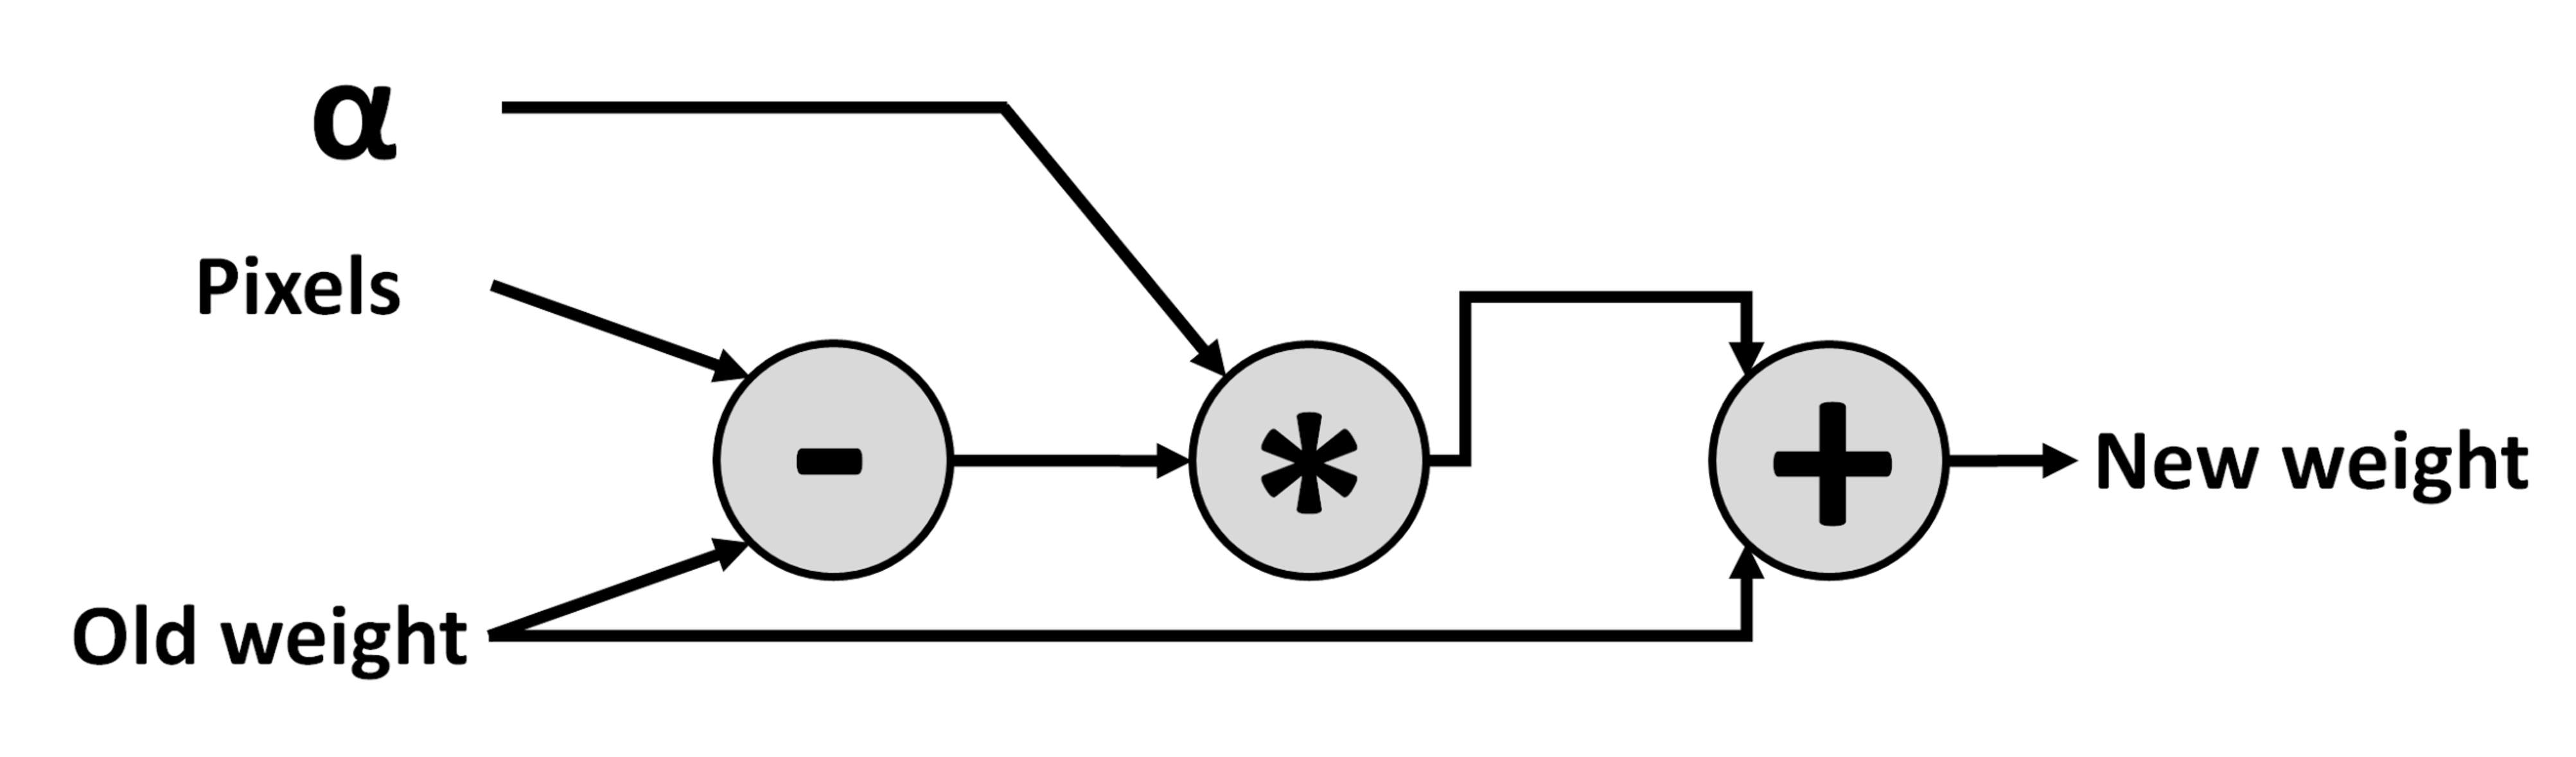
\includegraphics[width=0.9\columnwidth]{Weight_update}}
				\hfill
				\subcaptionbox
				{
					Output evaluate component
					\label{fig:output:evaluate}
				}
				{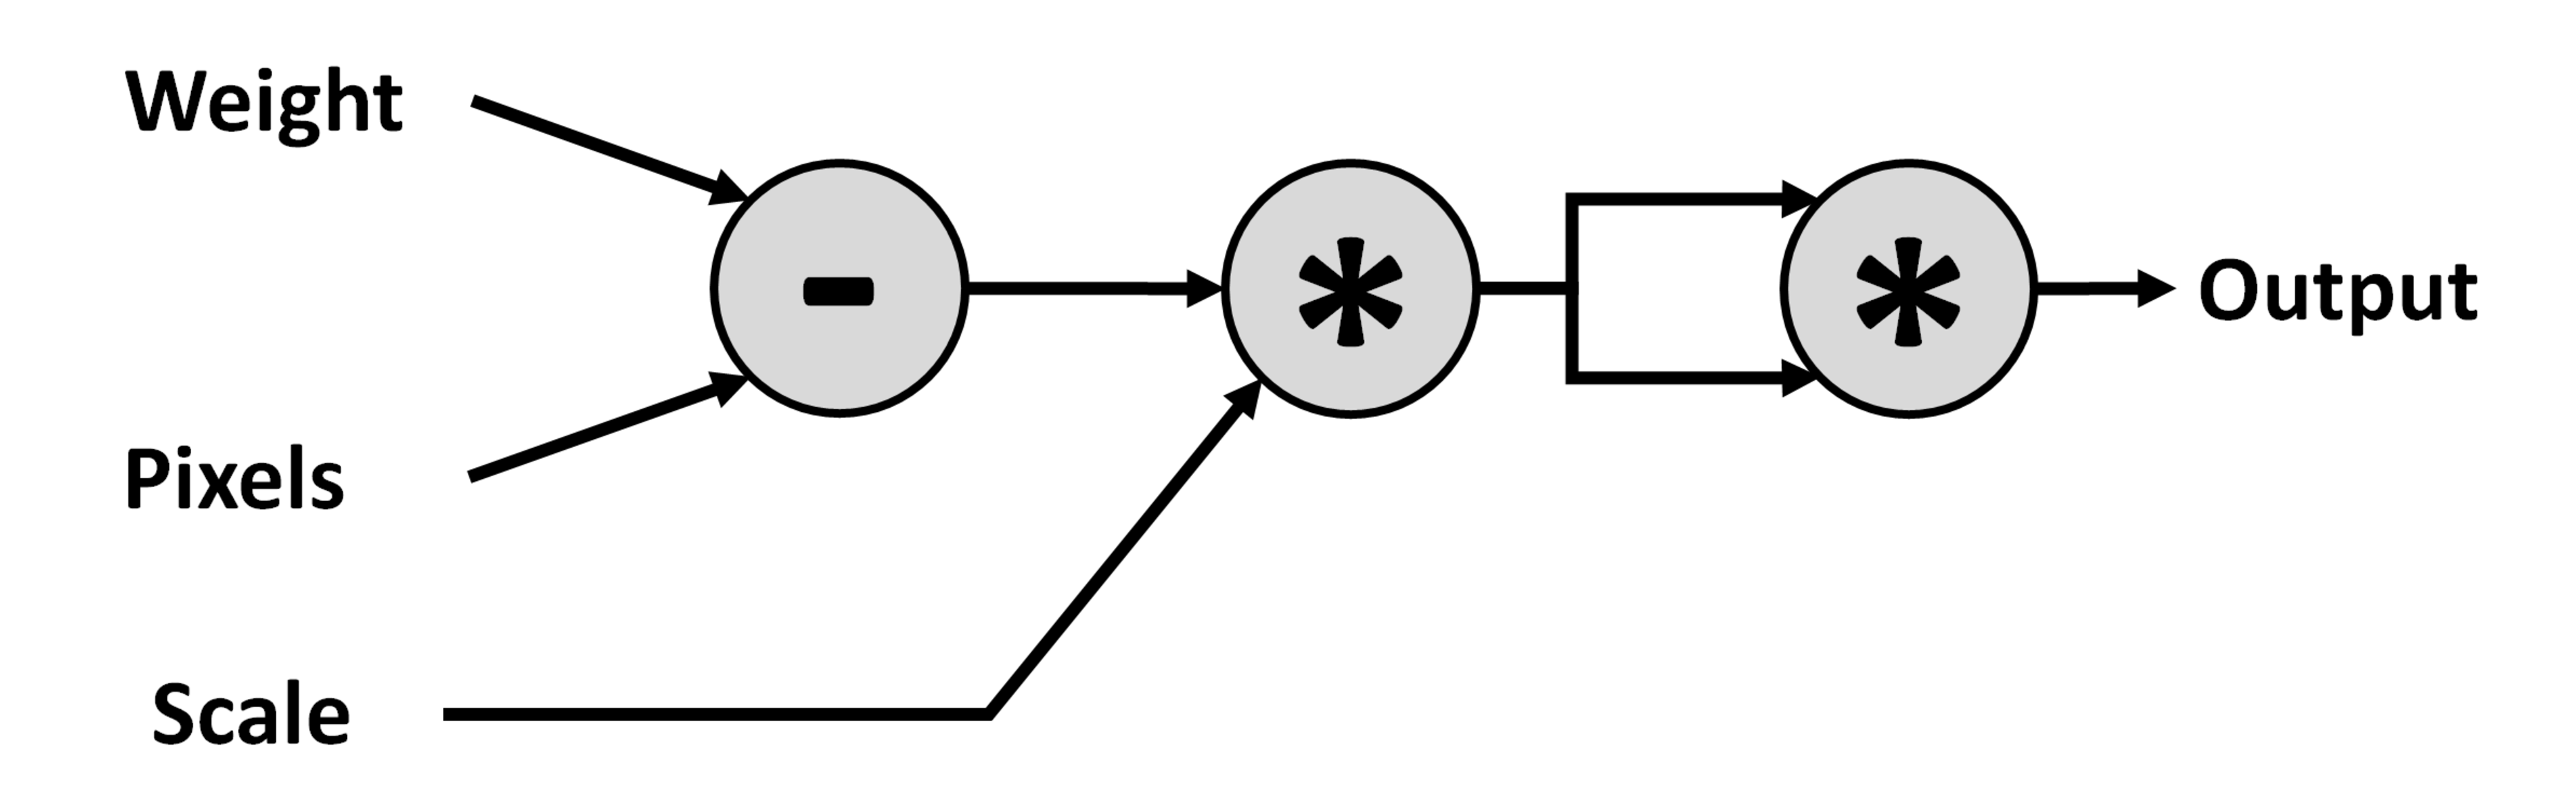
\includegraphics[width=0.9\columnwidth]{Ouput_evaluate}}
				\hfill
				\caption{Hardware computational elements, consisting of an LFSR \subfig{fig:lfsr}, weight update component \subfig{fig:weight:update}, and an output evaluate component \subfig{fig:output:evaluate}. The weight update block consists of stacked weight update components. The output evaluate blocks consists of output evaluate components connected to an adder tree.}
				\label{fig:computational_elements}
			\end{figure}
			
			As previously explained, the system utilizes two identical networks (one for males and one for females). The hardware model exploits this to reduce the size and power of the design by almost 50~\%. This was achieved by sharing the calculation blocks while storing the weight values separately. A drawback to this approach is that it reduces the testing performance by 50~\%, but since the major design constraints were area and power, this was an acceptable loss. Additionally, sharing those blocks induced some overhead, as control signals were required to synchronize the pipeline between the networks. The network select block was designed for that purpose.
			
			That network select block is a clock divider set to be half of the system clock frequency. Its output is used as a select signal for the multiplexer at the input of the output evaluate block, which is used to allow selection between the two networks. Additionally, that signal is used as an enable signal for the register at the output of the output evaluate block, which is used to store the output value of the male network. The output of that register and the output of the output evaluate block are connected to a comparator to perform the classification.
	
	\subsection{Results}
		The hardware design was initially tested in ModelSim. The same training and testing strategy used in the software were used for the hardware. Typical results are shown in \tbl{table:accuracy_results}, where the final accuracies, along with their corresponding standard deviations, were obtained after 30 training epochs across 10 iterations. The accuracies are similar amongst the different implementations, with the ideal accuracy being 70~\%. The hardware accuracies were able to reach that; however, they were typically lower and could be as much as 7~\% lower, depending on the weight initialization. This high degree of variance is due to the loss of precision with only 11 fractional bits. This is loosely shown in \fig{fig:sw_fractional_bits:testing}, where once the number of fractional bits reaches 12 the amount of variance decreases drastically. Based off these results, 12 or more fractional bits would have been a better alternative.
		
		The hardware design was synthesized with Synopsis' DC Compiler for TSMC018 process. The footprint of the design was 0.0176 mm\textsuperscript{2}. The total power of the system was measured to be 31.6 mW across all 30 epochs, resulting in a power consumption of 1.1 mW divided across 800 training and 1000 testing patterns (800 training + 200 testing). The area and power are both low, making this design suitable for embedded applications. Additional optimizations to both can be obtained. To improve the power the training and testing portions of the network could be disabled while they are not used. To improve the area a fully pipelined approach could be implemented, where only a single (or a few) functional components are used vs. an entire block of them.
		
		The system was able to process a pattern in as few as two clock cycles (for both the training and testing phases). A clock period of 20~ns was used, allowing for a new pattern to be processed after only 40~ns. Additionally, the clock was not optimized, so it is possible that the system can operate at a faster rate. Additional performance was not necessary for performing real-time gender classification, so that level of optimization was not performed.
		
		\begin{table}[!t]
			\renewcommand{\arraystretch}{1.3}
			\caption{Accuracies for the Hardware and Software Models After 30 Epochs}
			\label{table:accuracy_results}
			\centering
			\begin{tabular}{lcc}
				\hline
				Design                  & Train Accuracy           & Test Accuracy          \\
				\hline
				Ideal Software Model    & 70.125 \(\pm\) 0.000~\% & 70.000 \(\pm\) 0.000~\% \\
				Hardware Software Model & 66.150 \(\pm\) 0.378~\% & 64.200 \(\pm\) 0.812~\% \\
				Hardware Implementation & 68.363 \(\pm\) 0.401~\% & 67.850 \(\pm\) 0.950~\% \\
				\hline
			\end{tabular}
		\end{table}		
	
	\section{Conclusion}
		A CLC was implemented in both software and hardware to perform gender classification. A test accuracy of up to 70~\% was obtained for the ideal software model. Due to the loss of precision in the hardware implementation, the accuracies were typically lower; however, with an optimal weight initialization similar accuracies could be obtained. The synthesized area of the hardware was 0.0176 mm\textsuperscript{2}. The hardware consumed 1.1 mW of power per epoch per 800 training and 1000 testing patterns. Both training and testing can operate at a rate of at least 25~MHz.
		
		Given the extremely small size, low power consumption, and fast operation this design is suitable for real-time embedded applications. The performance is still many orders of magnitude faster than it would need to be for a simple marketing application. With that in mind, this design could be improved by performing power and area optimizations, such as disabling unused hardware and reducing the degree of parallelism. Additionally, the number of fractional bits could be increased to reduce the variance in the classification accuracy.
	
	% Bibliography
	\bibliographystyle{IEEEtran}
		% \IEEEtriggeratref{1}
		\bibliography{IEEEabrv,lfw}
	
\end{document}